
%% bare_jrnl.tex
%% V1.4b
%% 2015/08/26
%% by Michael Shell
%% see http://www.michaelshell.org/
%% for current contact information.
%%
%% This is a skeleton file demonstrating the use of IEEEtran.cls
%% (requires IEEEtran.cls version 1.8b or later) with an IEEE
%% journal paper.
%%
%% Support sites:
%% http://www.michaelshell.org/tex/ieeetran/
%% http://www.ctan.org/pkg/ieeetran
%% and
%% http://www.ieee.org/

%%*************************************************************************
%% Legal Notice:
%% This code is offered as-is without any warranty either expressed or
%% implied; without even the implied warranty of MERCHANTABILITY or
%% FITNESS FOR A PARTICULAR PURPOSE! 
%% User assumes all risk.
%% In no event shall the IEEE or any contributor to this code be liable for
%% any damages or losses, including, but not limited to, incidental,
%% consequential, or any other damages, resulting from the use or misuse
%% of any information contained here.
%%
%% All comments are the opinions of their respective authors and are not
%% necessarily endorsed by the IEEE.
%%
%% This work is distributed under the LaTeX Project Public License (LPPL)
%% ( http://www.latex-project.org/ ) version 1.3, and may be freely used,
%% distributed and modified. A copy of the LPPL, version 1.3, is included
%% in the base LaTeX documentation of all distributions of LaTeX released
%% 2003/12/01 or later.
%% Retain all contribution notices and credits.
%% ** Modified files should be clearly indicated as such, including  **
%% ** renaming them and changing author support contact information. **
%%*************************************************************************


% *** Authors should verify (and, if needed, correct) their LaTeX system  ***
% *** with the testflow diagnostic prior to trusting their LaTeX platform ***
% *** with production work. The IEEE's font choices and paper sizes can   ***
% *** trigger bugs that do not appear when using other class files.       ***                          ***
% The testflow support page is at:
% http://www.michaelshell.org/tex/testflow/



\documentclass[journal]{IEEEtran}
%
% If IEEEtran.cls has not been installed into the LaTeX system files,
% manually specify the path to it like:
% \documentclass[journal]{../sty/IEEEtran}





% Some very useful LaTeX packages include:
% (uncomment the ones you want to load)


% *** MISC UTILITY PACKAGES ***
%
%\usepackage{ifpdf}
% Heiko Oberdiek's ifpdf.sty is very useful if you need conditional
% compilation based on whether the output is pdf or dvi.
% usage:
% \ifpdf
%   % pdf code
% \else
%   % dvi code
% \fi
% The latest version of ifpdf.sty can be obtained from:
% http://www.ctan.org/pkg/ifpdf
% Also, note that IEEEtran.cls V1.7 and later provides a builtin
% \ifCLASSINFOpdf conditional that works the same way.
% When switching from latex to pdflatex and vice-versa, the compiler may
% have to be run twice to clear warning/error messages.






% *** CITATION PACKAGES ***
%
\usepackage{cite}
% cite.sty was written by Donald Arseneau
% V1.6 and later of IEEEtran pre-defines the format of the cite.sty package
% \cite{} output to follow that of the IEEE. Loading the cite package will
% result in citation numbers being automatically sorted and properly
% "compressed/ranged". e.g., [1], [9], [2], [7], [5], [6] without using
% cite.sty will become [1], [2], [5]--[7], [9] using cite.sty. cite.sty's
% \cite will automatically add leading space, if needed. Use cite.sty's
% noadjust option (cite.sty V3.8 and later) if you want to turn this off
% such as if a citation ever needs to be enclosed in parenthesis.
% cite.sty is already installed on most LaTeX systems. Be sure and use
% version 5.0 (2009-03-20) and later if using hyperref.sty.
% The latest version can be obtained at:
% http://www.ctan.org/pkg/cite
% The documentation is contained in the cite.sty file itself.






% *** GRAPHICS RELATED PACKAGES ***
%
\ifCLASSINFOpdf
  \usepackage[pdftex]{graphicx}
  % declare the path(s) where your graphic files are
  % \graphicspath{{../pdf/}{../jpeg/}}
  % and their extensions so you won't have to specify these with
  % every instance of \includegraphics
  \DeclareGraphicsExtensions{.pdf,.jpeg,.png,.eps,}
\else
  % or other class option (dvipsone, dvipdf, if not using dvips). graphicx
  % will default to the driver specified in the system graphics.cfg if no
  % driver is specified.
  % \usepackage[dvips]{graphicx}
  % declare the path(s) where your graphic files are
  % \graphicspath{{../eps/}}
  % and their extensions so you won't have to specify these with
  % every instance of \includegraphics
  % \DeclareGraphicsExtensions{.eps}
\fi
% graphicx was written by David Carlisle and Sebastian Rahtz. It is
% required if you want graphics, photos, etc. graphicx.sty is already
% installed on most LaTeX systems. The latest version and documentation
% can be obtained at: 
% http://www.ctan.org/pkg/graphicx
% Another good source of documentation is "Using Imported Graphics in
% LaTeX2e" by Keith Reckdahl which can be found at:
% http://www.ctan.org/pkg/epslatex
%
% latex, and pdflatex in dvi mode, support graphics in encapsulated
% postscript (.eps) format. pdflatex in pdf mode supports graphics
% in .pdf, .jpeg, .png and .mps (metapost) formats. Users should ensure
% that all non-photo figures use a vector format (.eps, .pdf, .mps) and
% not a bitmapped formats (.jpeg, .png). The IEEE frowns on bitmapped formats
% which can result in "jaggedy"/blurry rendering of lines and letters as
% well as large increases in file sizes.
%
% You can find documentation about the pdfTeX application at:
% http://www.tug.org/applications/pdftex

\usepackage{afterpage}



% *** MATH PACKAGES ***
%
\usepackage{amsmath}
% A popular package from the American Mathematical Society that provides
% many useful and powerful commands for dealing with mathematics.
%
% Note that the amsmath package sets \interdisplaylinepenalty to 10000
% thus preventing page breaks from occurring within multiline equations. Use:
%\interdisplaylinepenalty=2500
% after loading amsmath to restore such page breaks as IEEEtran.cls normally
% does. amsmath.sty is already installed on most LaTeX systems. The latest
% version and documentation can be obtained at:
% http://www.ctan.org/pkg/amsmath





% *** SPECIALIZED LIST PACKAGES ***
%
\usepackage{algorithmicx}
\usepackage{algorithm}
\usepackage{algpseudocode}
% algorithmic.sty was written by Peter Williams and Rogerio Brito.
% This package provides an algorithmic environment fo describing algorithms.
% You can use the algorithmic environment in-text or within a figure
% environment to provide for a floating algorithm. Do NOT use the algorithm
% floating environment provided by algorithm.sty (by the same authors) or
% algorithm2e.sty (by Christophe Fiorio) as the IEEE does not use dedicated
% algorithm float types and packages that provide these will not provide
% correct IEEE style captions. The latest version and documentation of
% algorithmic.sty can be obtained at:
% http://www.ctan.org/pkg/algorithms
% Also of interest may be the (relatively newer and more customizable)
% algorithmicx.sty package by Szasz Janos:
% http://www.ctan.org/pkg/algorithmicx




% *** ALIGNMENT PACKAGES ***
%
\usepackage{array}
% Frank Mittelbach's and David Carlisle's array.sty patches and improves
% the standard LaTeX2e array and tabular environments to provide better
% appearance and additional user controls. As the default LaTeX2e table
% generation code is lacking to the point of almost being broken with
% respect to the quality of the end results, all users are strongly
% advised to use an enhanced (at the very least that provided by array.sty)
% set of table tools. array.sty is already installed on most systems. The
% latest version and documentation can be obtained at:
% http://www.ctan.org/pkg/array


% IEEEtran contains the IEEEeqnarray family of commands that can be used to
% generate multiline equations as well as matrices, tables, etc., of high
% quality.




% *** SUBFIGURE PACKAGES ***
%\ifCLASSOPTIONcompsoc
%  \usepackage[caption=false,font=normalsize,labelfont=sf,textfont=sf]{subfig}
%\else
  \usepackage[caption=false,font=footnotesize]{subfig}
%\fi
% subfig.sty, written by Steven Douglas Cochran, is the modern replacement
% for subfigure.sty, the latter of which is no longer maintained and is
% incompatible with some LaTeX packages including fixltx2e. However,
% subfig.sty requires and automatically loads Axel Sommerfeldt's caption.sty
% which will override IEEEtran.cls' handling of captions and this will result
% in non-IEEE style figure/table captions. To prevent this problem, be sure
% and invoke subfig.sty's "caption=false" package option (available since
% subfig.sty version 1.3, 2005/06/28) as this is will preserve IEEEtran.cls
% handling of captions.
% Note that the Computer Society format requires a larger sans serif font
% than the serif footnote size font used in traditional IEEE formatting
% and thus the need to invoke different subfig.sty package options depending
% on whether compsoc mode has been enabled.
%
% The latest version and documentation of subfig.sty can be obtained at:
% http://www.ctan.org/pkg/subfig




% *** FLOAT PACKAGES ***
%
%\usepackage{fixltx2e}
% fixltx2e, the successor to the earlier fix2col.sty, was written by
% Frank Mittelbach and David Carlisle. This package corrects a few problems
% in the LaTeX2e kernel, the most notable of which is that in current
% LaTeX2e releases, the ordering of single and double column floats is not
% guaranteed to be preserved. Thus, an unpatched LaTeX2e can allow a
% single column figure to be placed prior to an earlier double column
% figure.
% Be aware that LaTeX2e kernels dated 2015 and later have fixltx2e.sty's
% corrections already built into the system in which case a warning will
% be issued if an attempt is made to load fixltx2e.sty as it is no longer
% needed.
% The latest version and documentation can be found at:
% http://www.ctan.org/pkg/fixltx2e


\usepackage{stfloats}
% stfloats.sty was written by Sigitas Tolusis. This package gives LaTeX2e
% the ability to do double column floats at the bottom of the page as well
% as the top. (e.g., "\begin{figure*}[!b]" is not normally possible in
% LaTeX2e). It also provides a command:
%\fnbelowfloat
% to enable the placement of footnotes below bottom floats (the standard
% LaTeX2e kernel puts them above bottom floats). This is an invasive package
% which rewrites many portions of the LaTeX2e float routines. It may not work
% with other packages that modify the LaTeX2e float routines. The latest
% version and documentation can be obtained at:
% http://www.ctan.org/pkg/stfloats
% Do not use the stfloats baselinefloat ability as the IEEE does not allow
% \baselineskip to stretch. Authors submitting work to the IEEE should note
% that the IEEE rarely uses double column equations and that authors should try
% to avoid such use. Do not be tempted to use the cuted.sty or midfloat.sty
% packages (also by Sigitas Tolusis) as the IEEE does not format its papers in
% such ways.
% Do not attempt to use stfloats with fixltx2e as they are incompatible.
% Instead, use Morten Hogholm'a dblfloatfix which combines the features
% of both fixltx2e and stfloats:
%
%\usepackage{dblfloatfix}
% The latest version can be found at:
% http://www.ctan.org/pkg/dblfloatfix




\ifCLASSOPTIONcaptionsoff
  \usepackage[nomarkers]{endfloat}
  \let\MYoriglatexcaption\caption
  \renewcommand{\caption}[2][\relax]{\MYoriglatexcaption[#2]{#2}}
\fi
% endfloat.sty was written by James Darrell McCauley, Jeff Goldberg and 
% Axel Sommerfeldt. This package may be useful when used in conjunction with 
% IEEEtran.cls'  captionsoff option. Some IEEE journals/societies require that
% submissions have lists of figures/tables at the end of the paper and that
% figures/tables without any captions are placed on a page by themselves at
% the end of the document. If needed, the draftcls IEEEtran class option or
% \CLASSINPUTbaselinestretch interface can be used to increase the line
% spacing as well. Be sure and use the nomarkers option of endfloat to
% prevent endfloat from "marking" where the figures would have been placed
% in the text. The two hack lines of code above are a slight modification of
% that suggested by in the endfloat docs (section 8.4.1) to ensure that
% the full captions always appear in the list of figures/tables - even if
% the user used the short optional argument of \caption[]{}.
% IEEE papers do not typically make use of \caption[]'s optional argument,
% so this should not be an issue. A similar trick can be used to disable
% captions of packages such as subfig.sty that lack options to turn off
% the subcaptions:
% For subfig.sty:
% \let\MYorigsubfloat\subfloat
% \renewcommand{\subfloat}[2][\relax]{\MYorigsubfloat[]{#2}}
% However, the above trick will not work if both optional arguments of
% the \subfloat command are used. Furthermore, there needs to be a
% description of each subfigure *somewhere* and endfloat does not add
% subfigure captions to its list of figures. Thus, the best approach is to
% avoid the use of subfigure captions (many IEEE journals avoid them anyway)
% and instead reference/explain all the subfigures within the main caption.
% The latest version of endfloat.sty and its documentation can obtained at:
% http://www.ctan.org/pkg/endfloat
%
% The IEEEtran \ifCLASSOPTIONcaptionsoff conditional can also be used
% later in the document, say, to conditionally put the References on a 
% page by themselves.




% *** PDF, URL AND HYPERLINK PACKAGES ***
%
\usepackage{url}
% url.sty was written by Donald Arseneau. It provides better support for
% handling and breaking URLs. url.sty is already installed on most LaTeX
% systems. The latest version and documentation can be obtained at:
% http://www.ctan.org/pkg/url
% Basically, \url{my_url_here}.




% *** Do not adjust lengths that control margins, column widths, etc. ***
% *** Do not use packages that alter fonts (such as pslatex).         ***
% There should be no need to do such things with IEEEtran.cls V1.6 and later.
% (Unless specifically asked to do so by the journal or conference you plan
% to submit to, of course. )


% correct bad hyphenation here
\hyphenation{op-tical net-works semi-conduc-tor}


\begin{document}
%
% paper title
% Titles are generally capitalized except for words such as a, an, and, as,
% at, but, by, for, in, nor, of, on, or, the, to and up, which are usually
% not capitalized unless they are the first or last word of the title.
% Linebreaks \\ can be used within to get better formatting as desired.
% Do not put math or special symbols in the title.
\title{Mitigating Catastrophic Forgetting in Space Communications Cognitive Engine}
%
%
% author names and IEEE memberships
% note positions of commas and nonbreaking spaces ( ~ ) LaTeX will not break
% a structure at a ~ so this keeps an author's name from being broken across
% two lines.
% use \thanks{} to gain access to the first footnote area
% a separate \thanks must be used for each paragraph as LaTeX2e's \thanks
% was not built to handle multiple paragraphs
%

\author{Max~Li,
		Timothy~M.~Hackett,
        Sven~G.~Bil\'{e}n,\textit{~Senior~Member,~IEEE,}
        Paulo~Victor~R.~Ferreira,
        Alexander~M.~Wyglinski,\textit{~Senior~Member,~IEEE,}
        Richard~C.~Reinhart,
        and~Dale~J.~Mortensen%
        
\thanks{T. Hackett and S. Bil\'{e}n are with the School
of Electrical Engineering and Computer Science, The Pennsylvania State University, University Park, PA 16801, USA, \{Email: tmh5344@psu.edu, sbilen@psu.edu\}}%
\thanks{M.Li, P. Ferreira and A. Wyglinski are with the Department of Electrical Engineering \& Computer Engineering, Worcester Polytechnic Institute, Worcester, MA 01609, USA, \{Email: mhli@wpi.edu,prferreira@wpi.edu, alexw@wpi.edu\}}%
\thanks{R. Reinhart and D. Mortensen are with NASA John H. Glenn Research Center, Cleveland, OH 44135, USA, \{Email: richard.c.reinhart@nasa.gov, dale.mortensen@nasa.gov\}}%
\thanks{Manuscript received ; revised .}}

% note the % following the last \IEEEmembership and also \thanks - 
% these prevent an unwanted space from occurring between the last author name
% and the end of the author line. i.e., if you had this:
% 
% \author{....lastname \thanks{...} \thanks{...} }
%                     ^------------^------------^----Do not want these spaces!
%
% a space would be appended to the last name and could cause every name on that
% line to be shifted left slightly. This is one of those "LaTeX things". For
% instance, "\textbf{A} \textbf{B}" will typeset as "A B" not "AB". To get
% "AB" then you have to do: "\textbf{A}\textbf{B}"
% \thanks is no different in this regard, so shield the last } of each \thanks
% that ends a line with a % and do not let a space in before the next \thanks.
% Spaces after \IEEEmembership other than the last one are OK (and needed) as
% you are supposed to have spaces between the names. For what it is worth,
% this is a minor point as most people would not even notice if the said evil
% space somehow managed to creep in.



% The paper headers
\markboth{IEEE Transactions on Cognitive Communications and Networking,~Vol.~, No.~, Month~2019}%
{Shell \MakeLowercase{\textit{et al.}}: Bare Demo of IEEEtran.cls for IEEE Journals}
% The only time the second header will appear is for the odd numbered pages
% after the title page when using the twoside option.
% 
% *** Note that you probably will NOT want to include the author's ***
% *** name in the headers of peer review papers.                   ***
% You can use \ifCLASSOPTIONpeerreview for conditional compilation here if
% you desire.




% If you want to put a publisher's ID mark on the page you can do it like
% this:
\IEEEoverridecommandlockouts
\IEEEpubid{\makebox[\columnwidth]{978-1-5386-3988-7/17/\$31.00~
\copyright2018
IEEE \hfill} \hspace{\columnsep}\makebox[\columnwidth]{ }}



% use for special paper notices
%\IEEEspecialpapernotice{(Invited Paper)}




% make the title area
\maketitle

% As a general rule, do not put math, special symbols or citations
% in the abstract or keywords.
\begin{abstract}
TODO:
Cognitive algorithms for communications systems have been presented in literature, but very few have been integrated into a fielded system, especially space communications systems.  In this paper, we describe the implementation of a multi-objective reinforcement-learning algorithm using deep artificial neural networks acting as a radio-resource-allocation controller.  The developed software core is generic in nature and can be ported readily to another application.  The cognitive engine algorithm implementation was characterized through a series of tests using both a ground-based system and a space-based system.  The ground system comprised of engineering-model software-defined radios, commercial modems, and RF equipment emulating the targeted space-to-ground channel.  The on-orbit communication system, including a space-based, remotely controlled transmitter, resides on the International Space Station and operates with a ground-based receiver at NASA Glenn Research Center.  Through a series of on-orbit tests, the cognitive engine was tested in a highly dynamic channel and its performance is discussed and analyzed.
\end{abstract}

% Note that keywords are not normally used for peerreview papers.
\begin{IEEEkeywords}
TODO:
\end{IEEEkeywords}






% For peer review papers, you can put extra information on the cover
% page as needed:
% \ifCLASSOPTIONpeerreview
% \begin{center} \bfseries EDICS Category: 3-BBND \end{center}
% \fi
%
% For peerreview papers, this IEEEtran command inserts a page break and
% creates the second title. It will be ignored for other modes.
\IEEEpeerreviewmaketitle


\parskip=0pt
\section{Introduction} \label{sec:introduction}
\begin{itemize}
	\item Motivate CR / discuss ISS work and testing
	\item previous work, multi-objective nature
	\item architecture runs into catastrophic forgetting, as explained in section sec:catforget or whatever.
	\item ensemble based, recursive based methods implemented, tested on flight as follow on to [tim's stuff]
\end{itemize}
\IEEEPARstart{C}{omputing} performance continues to increase with every new generation of general purpose processors (GPPs), graphics processing units (GPUs), and field-programmable gate arrays (FPGAs).  This makes the use of software-defined radios (SDRs) increasingly feasible for space communications applications \cite{reinhart-sdr,sdr-arch-morlet}.  Cognitive communication algorithms have been proposed in the past, but many of those implemented and tested often have employed dynamic spectrum access techniques or other sensing approaches.  These new technologies strive to achieve multi-objective goals by modifying multiple radio parameters through rewarded behavior and provides the foundation for deploying cognitive systems, especially for autonomous space applications.

The International Space Station (ISS) currently hosts three SDRs on a research platform called the Space Communications and Navigation (SCaN) Testbed \cite{reinhart-paper}.  NASA is interested in characterizing the applicability of SDRs for future missions in terms of new operational aspects, new software development paradigms (as opposed to building specialized hardware), and the ability to change the signal waveforms \cite{ta05}.  This paper describes the implementation and testing of a ground-based space communications cognitive engine (CE) that controls an S-band radio on the SCaN Testbed along with ground SDRs and commercial modems in order to test the proposed multi-objective reinforcement learning (MORL) using deep neural networks algorithm for use as a radio-resource-allocation controller outlined in \cite{paulo-jrnl}.

NASA's SCaN Testbed experimental state-of-the-art communication system consists of an adaptive coding and modulation scheme, which changes the transmitter parameters through the use of a lookup table with closed-loop feedback.  The ground receiver senses the signal-to-noise (SNR) or \textit{E}\textsubscript{s}/\textit{N}\textsubscript{0} (energy per symbol to noise power spectral density ratio) level and then looks at a pre-generated table that provides the optimal modulation-coding pair (MODCOD) for that given signal quality.  The chosen MODCOD is then sent through a control channel back to the space transmitter to update its properties for the next transmitted frame.  This table is generally built to maintain quasi-error-free performance in an additive white Gaussian noise (AWGN) channel.  The table is developed by a team of experts that runs series of tests to characterize the radio's performance.  This type of adaptive communications is a bi-objective radio-resource-allocation optimization, in which the two balancing objectives are throughput and frame error rate (FER).  The authors' proposed reinforcement-learning neural network algorithm (RLNN2) in \cite{paulo-jrnl} is, in a sense, the generalization of the developed adaptive communications model, allowing for more flexibility in terms of adaptation and achievement of multiple goals at the cost of computational power.  Instead of just balancing between minimizing FER and maximizing throughput, the proposed algorithm can handle any number of objectives, such as FER, throughput, occupied bandwidth, spectral efficiency, transmit power efficiency, and DC power consumption.  Likewise, in addition to just the MODCOD, our proposed RLNN2 algorithm has the ability to change the transmit power, filter roll-off factor, and symbol rate to meet these objectives.  In contrast to the static table used in the adaptive architecture, the CE \textit{learns} (using reinforcement learning) the optimal transmission parameters (referred to as ``action tuples'') given the sensed \textit{E}\textsubscript{s}/\textit{N}\textsubscript{0}.

\begin{algorithm}
 	\caption{RLNN2 operational routine adapted from \cite{paulo-jrnl}.}
 	\label{RLNN2_algorithm_1}
 	\begin{algorithmic}[1] 		
 		\Require{NN1 and NN2 setup, and $\bar{R_{\textrm{s}}}$, $\bar{E_{\textrm{s}}}$, $\bar{k}$, $\bar{\beta}$, $\bar{M}$, $\bar{c}$, $\textrm{NN}_{\textrm{bs}}$, $\textrm{NN}_{\textrm{dump}}$, $f(\varepsilon)$, $\textrm{tr}_{a}$, $\textrm{min}_{\mathrm{good}\%}$}
 		\State $\textbf{U} \gets$ all combinations of $(\bar{R_{\textrm{s}}}, \bar{E_{\textrm{s}}}, \bar{k}, \bar{\beta}, \bar{M}, \bar{c})$
 		

 		\Loop
 		\If {$(\bar{R_{\textrm{s}}}, \bar{E_{\textrm{s}}}, \bar{k}, \bar{\beta}, \bar{M}, \bar{c})$ has changed}
 			\State $\textbf{U} \gets$ all combinations of $(\bar{R_{\textrm{s}}}, \bar{E_{\textrm{s}}}, \bar{k}, \bar{\beta}, \bar{M}, \bar{c})$
 		\EndIf
 		
 		\While {NN training data buffer not full}
 			\State `Forced exploration': only explore
 		\EndWhile 		
 		\State z~$\gets$ uniform random number $[0, 1]$
 		\If {z~$<f(\varepsilon)=\varepsilon_{k}$} \Comment{with prob.~$\varepsilon_{k}$~(Explore)}
			\State Predict actions using NN1
			\State Classify actions into good or bad using $\textrm{min}_{\textrm{good}\%}$
			\State u~$\gets$ uniform random number $[0, 1]$ 
			\If {u$<\textrm{tr}_{a}$} \Comment{Action rejection}
				\State Randomly select one good action $a$
			\Else
 				\State Randomly select one bad action $a$
 			\EndIf
 		\Else \Comment{with probability~$1-\varepsilon_{k}$~(Exploit)}
 			\State Predict action to be exploited using NN2
 			\State Execute selected $a$
 			\State Measure and/or read RL states $\bar{s}$
 			\State Compute multi-objective fitness function $f_{\textrm{obs}}(x)$
 			\State Select next $\textrm{NN2}_{\textrm{input}}$
 			\State Update NN training data buffer
 			\State Build NN1 and NN2 training datasets
 			\If {NN training data buffer is full} 
 				\State Remove $\textrm{NN}_{\textrm{dump}}$ entries from NN training dataset
 			\EndIf
 		\EndIf
 		\EndLoop
 	\end{algorithmic}
 \end{algorithm}
 \begin{table}[h]
 \caption{Algorithm~1 Nomenclature}
 \begin{center}
   \begin{tabular}{l|l}
		\hline		
		Symbol & Description	\\	
		\hline
		$\bar{\beta}$ & Filter roll-off factor\\		
		$\bar{c}$ & Encoding rate\\		
		$\bar{E_{\textrm{s}}}$ & Additional TX \textit{E}\textsubscript{s}/\textit{N}\textsubscript{0}\\
		$f(\varepsilon)$ & Explore probability function\\
		$\bar{k}$ & Bits per symbol\\
		$\bar{M}$ & Modulation order\\
		$\textrm{min}_{\mathrm{good}\%}$ & Virtual exploration performance bin threshold\\
		$\textrm{NN1}$ & Explore NN ensemble \\
		$\textrm{NN2}$ & Exploit NN ensemble \\
		$\textrm{NN}_{\textrm{bs}}$ & NN buffer size\\
		$\textrm{NN}_{\textrm{dump}}$ & Number of buffer entries pruned after  training\\
		$\bar{R_{\textrm{s}}}$ & Symbol rate \\
		$\textrm{tr}_{a}$ & Action rejection threshold\\
		\hline
	\end{tabular}
\end{center}
 \end{table}


To demonstrate the RLNN2 algorithm within a space communications architecture, we have chosen to leverage the existing architecture used in \cite{downey-paper} since it decreased the development time and risk.  This setup is described in more detail in Section~\ref{sec:flight-testing-test-setup}.  The adaptive workstation that provides the lookup table was replaced with a workstation containing our RLNN2 cognitive algorithm.  As in \cite{downey-paper}, our implementation of the RLNN2 algorithm was designed to be operated with the Digital Video Broadcasting--Satellite--Second Generation (DVB-S2) standard \cite{dvbs2-standard}, a widely available commercial broadcast satellite waveform with a bank of MODCODs available to use as link conditions allow.  The waveform provides QPSK, 8-PSK, 16-APSK, and 32-APSK modulation schemes; BCH+LDPC coding with effective coding rates of 0.18 to 0.87 using fixed-size short frames; and a square-root raised-cosine pulse-shape filter with factors of $\beta=\{0.2,0.25,0.35\}$.  It supports both variable coding and modulation (VCM) and adaptive coding and modulation (ACM) with an on-the-fly MODCOD and roll-off adaptations.  Unfortunately, the waveform does not support on-the-fly symbol rate changes, which means the implementation and test of the CE did not include an adaptive symbol rate.

% needed in second column of first page if using \IEEEpubid
\IEEEpubidadjcol

This paper provides details on porting the RLNN2 MATLAB algorithms presented in \cite{paulo-jrnl} into a fielded system, its characterization on the ground, and its performance in a real-world, challenging space-to-ground channel.  Section~II provides an overview of the mechanics of the CE.  Section~III provides a summary of the software implementation and architecture as first discussed by the authors in \cite{tim-ccaa}.  Section~IV describes the characterization of the CE using a ground system emulating the ISS-to-ground channel and using engineering-model SDRs.  Section~V provides the on-orbit experiment testing architecture, test schedule, and key analyses from the data gathered.  Finally, Section~VI provides a discussion of the results and provides many areas to be improved upon in future work.

\section{Overview of Cognitive Engine} \label{sec:overview}
\begin{figure}[t]
\centering
 \includegraphics[width=0.8\linewidth]{./figures/paulo-rlnn-diagram.eps}
 \caption{General flow block diagram of the RLNN2 (adapted from \cite{paulo-jrnl}).  On each iteration, the action parameters are updated either using virtual exploration or exploiting learned knowledge.}
 \label{fig:paulo-rlnn-diagram}
\end{figure}

The theoretical background and preliminary simulations for the multi-objective RLNN2 CE are described in detail in \cite{paulo-jrnl}, which builds upon \cite{paulo-ccaa-paper,aiaa-paulo}.  This section provides a brief introduction to the algorithms to provide context for the reader with respect to the remaining portion of this paper.  Algorithm~I (adapted from \cite{paulo-jrnl}) provides the RLNN2 operational routine.

The RLNN2 is a reinforcement learner that leverages neural networks for exploitation (as substitute for the RL Q-table) and exploration (for ``virtual'' exploration \cite{paulo-jrnl,paulo-ccaa-paper}).  The process flow of the algorithm is shown in Fig.~\ref{fig:paulo-rlnn-diagram}.  On each iteration, the CE can choose to exploit previous knowledge or explore new actions.  The probability of exploring uses a cyclic epsilon--greedy method, where the probability of exploring is $1/k$, where $k$ is an integer increasing by 1 on each iteration.  When $k=250$, $k$ is reset to 1.

The reinforcement learner as described in \cite{paulo-jrnl} follows a greedy policy given by
\begin{equation}
\pi(s) = \underset{a}{\text{argmax}} \,\,Q(s,a)\,,
\end{equation}
where $Q(s,a)$ represents the long-run value of being in state $s$ and performing action $a$.  The optimal policy at state $s$ is choosing the action that maximizes $Q(s,a)$.  A modified version of Bellman's equation is used for learning $Q(s,a)$ over time:
\begin{equation}
\begin{split}
Q_{k+1}(s_k(t),&a_k)= \\ &Q_k(s_k(t),a_k)+\alpha[r_k(t)-Q_k(s_k(t),a_k)]\,,
\end{split}
\end{equation}
where $r_k$ is the instantaneous reward and $\alpha$ is the learning rate.  The state $s_k(t)$ is a function of continuous time because of the dynamic nature of the channel conditions \cite{paulo-jrnl}.  As pointed out in \cite{aiaa-paulo}, for this online application, any action can be taken from any state without needing any planning, so consequently, the CE is only interested in the immediate reward.

The goal of this algorithm is to maximize the weighted sum of a set of multi-objective functions that characterize the performance of the radio.  In this proof-of-concept experiment, the following fitness functions were used as defined in \cite{paulo-jrnl}---the throughput computed by
\begin{equation}
f_\mathrm{Thrp} = R_\mathrm{s} k c\,,
\end{equation}
the bandwidth by
\begin{equation}
f_\mathrm{BW} = R_\mathrm{s}(1+\beta)\,,
\end{equation}
the spectral efficiency by
\begin{equation}
f_\mathrm{Spc\_eff} = kc/(1+\beta)\,,
\end{equation}
the power efficiency by
\begin{equation}
f_\mathrm{Pwr\_eff} = (kc)/(10^{E_\mathrm{s}/N_\mathrm{0}/10}R_\mathrm{s})\,,
\end{equation}
and the DC power consumed by
\begin{equation}
f_\mathrm{Pwr\_con} = E_\mathrm{s} R_\mathrm{s}\,,
\end{equation}
where $R_\mathrm{s}$ is the symbol rate, $k$ is the bits per symbol, $c$ is coding rate, $\beta$ is the pulse shaping filter roll-off factor, and $E_\mathrm{s}$ is the additional transmit energy (in dB) used over the minimum $E_\mathrm{s}/N_\mathrm{0}$.  The FER was computed by using FER vs. $E_\mathrm{s}/N_\mathrm{0}$ curves measured for the intended DVB-S2 ground modem by the authors of \cite{downey-paper} in previous work.  The weighted sum multi-objective fitness function is computed by:
\begin{equation}
\begin{split}
f_\mathrm{obs}(x) = &w_1 \bar{f}_\mathrm{Thrp} + w_2 \bar{f}_\mathrm{FER} + w_3 \bar{f}_\mathrm{BW} + \\
&w_4 \bar{f}_\mathrm{Spc\_eff} + w_5 \bar{f}_\mathrm{Pwr\_eff} + w_6 \bar{f}_\mathrm{Pwr\_con}\,,
\end{split}
\end{equation} 
where $\bar{f_i}$ is $f_i$ normalized to [0,1].  The RL reward, $r_k$, is defined as $f_\mathrm{obs}(x)$, where $x$ encompasses the weight vector $\bar{w}$ and all other parameters necessary to compute $f_\mathrm{obs}$.  Six different weight vectors were tested in ground testing (Table~\ref{table:ground_test_matrix} in Section~\ref{sec:ground-testing}), which represent different mission needs for communications.  Of these six, three were used in on-orbit testing (Table~\ref{table:flight_test_matrix} in Section~\ref{sec:flight-testing}).  As pointed out in \cite{paulo-jrnl}, the RL states are features of the aforementioned fitness function and the current environment state.  All environment changes are assumed to be conveyed by the satellite communications channel, which is measured as the SNR at the receiver.

The set of exploit NN ensembles takes in an input of the normalized performance values of each objective as well as the current \textit{E}\textsubscript{s}/\textit{N}\textsubscript{0} and outputs the action that corresponds to that performance given the \textit{E}\textsubscript{s}/\textit{N}\textsubscript{0}.  Each exploit NN ensemble outputs one of the elements in the action tuple (modulation scheme, encoding rate, filter roll-off factor, and transmit power).  The output of the NN ensemble is simply the mean of the member NNs.  Each individual exploit NN is a fully-connected feed-forward network without bias consisting of a 7-neuron-wide input layer, 20-neuron-wide hidden layer with a log--sigmoid activation function, and a 1-neuron output layer with a linear activation function.

The explore NN ensemble takes in an action tuple and the current \textit{E}\textsubscript{s}/\textit{N}\textsubscript{0} and outputs the fitness score weighted by the relative importance of each objective function.  Like the exploit ensembles, the output of the explore ensemble is the mean of the individual explore NNs.  Each explore NN network is a fully-connected feed-forward without bias consisting of a 7-neuron input; 7- and 50-neuron hidden layers using a log--sigmoid activation function; and 1-neuron output layer with a linear activation function.  Each possible action (or a subset of the entire action space) is sent to the explore NN ensemble to predict the performance of each action.  The performance values are thresholded into two bins: the ``good'' actions (which result in good performance) and the ``bad'' actions (which result in poor performance).  In the ground and flight experiments discussed in this paper, a threshold of 90\% of the maximum predicted Q-value was used---actions above this threshold were considered good actions and the rest were bad actions.  A random action (uniformly distributed) is then chosen from one of these bins based on the rejection probability hyperparameter (set to 95\%).  The rejection probability enables good actions to be chosen most of the time but allows for bad actions to be chosen occasionally.  The rationale for why the good actions are not always chosen is because the knowledge of the environment model in the NN is not complete---what it predicts as a bad action may actually be a good action.  This is known as virtual exploration \cite{paulo-ccaa-paper,paulo-jrnl}.

The action parameters are sent to the DVB-S2 transmitter, which changes its transmission parameters on the next frame.  The \textit{E}\textsubscript{s}/\textit{N}\textsubscript{0} and measured performances of FER, throughput, spectral efficiency, DC power consumption, and transmit power efficiency are recorded to a training buffer.  When the training buffer fills up over time, the explore and set of exploit NN ensembles are retrained using the Levenberg--Marquardt (LM) backpropagation algorithm \cite{levenberg-marquardt} based on the set of data in the training buffer \cite{paulo-jrnl}.  During training, 90\% of the data is used for training, and 10\% used for validation.  The same data are used for each NN in an ensemble with randomized orders.  For this iteration of the RLNN2 algorithm, the LM algorithm was chosen for backpropagation because of its simple training algorithm that works well with small data sets and quick convergence.  In this design iteration, it was desirable to be able execute and train online in real-time during a pass.  To achieve this goal, the network complexity and the training process had to be simple and quick.

\section{Software Implementation} \label{sec:softwareimplementation}
The software architecture for this CE was first introduced by the authors in \cite{tim-ccaa}.  This section provides a summary of the architecture as it applies to the ground testing and on-orbit testing results presented in later sections.

The performance of the proposed RLNN2 algorithms were assessed with MATLAB simulations, as described in \cite{paulo-jrnl}, for proof-of-concept purposes.  For experimentation with a real-world flight system, the CE was developed using an object-oriented architecture designed for performance, generality, and reuse.  The CE was developed in C++ leveraging some of the constructs in the C++11 standard \cite{c++11-standard} and many open-source software libraries to maximize performance and provide more capability to port the engine to different (possibly embedded) platforms.  The software was developed in a UNIX environment, but designed to be recompiled for any operating system.  Software libraries (described in Section~\ref{sec:softwarelibraries}) were used for the NNs, matrix algebra, external interfacing to the modems, and saving/restoring program sessions.

\subsection{Libraries} \label{sec:softwarelibraries}
\begin{figure*}[t]
\centering
 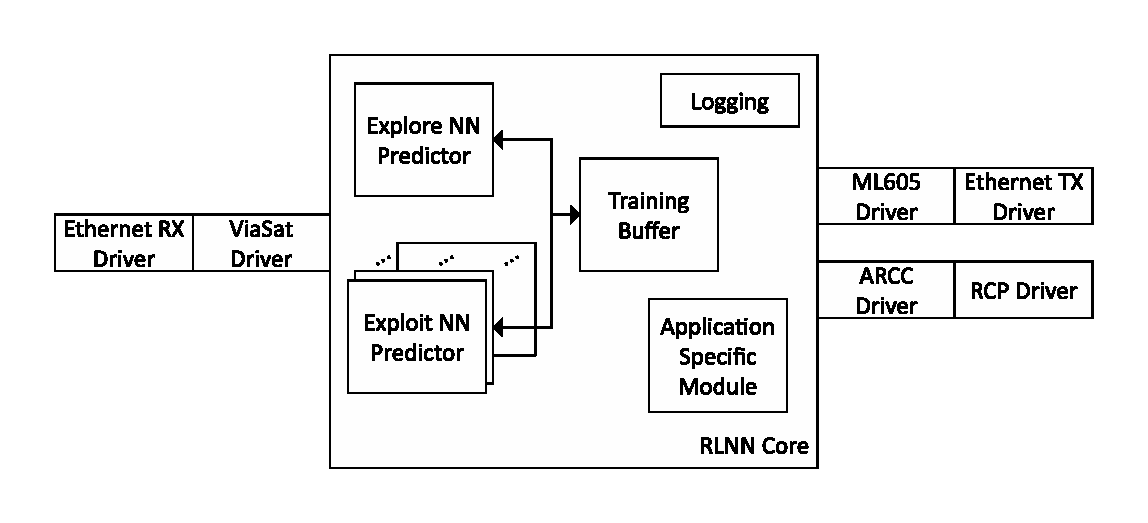
\includegraphics[width=0.75\linewidth]{./figures/software-arch.eps}
 \caption{Implemented software architecture of the RLNN2.  The RLNN2 Core hosts the RLNN2 algorithms; the drivers interface with the various receivers and transmitters.}
 \label{fig:soft-arch}
\end{figure*}

Each year, the number of publicly available artificial neural network (ANN) and machine learning libraries continues to expand.  Many of these libraries have application program interfaces (APIs) for high-level languages, such as Python, but lack APIs for lower-level languages, such as C/C++.  Furthermore, some of the C/C++ applicable libraries lack documentation for their lower-level APIs, possess very complex build processes \cite{caffe-documentation} (which eliminates portability to embedded devices), and/or were designed for very large, complex applications \cite{darknet-documentation} (such as deep, convolutional NNs).

MLPack \cite{mlpack-documentation} was chosen to implement the NNs in our CE.  At the time of developing our software, the ANN library was only available on the ``master'' branch on GitHub; it was not included in any of the stable releases.  It also did not include a Levenburg--Marquardt backpropagation implementation for training; hence, this functionality was written from scratch by the authors.

Armadillo \cite{armadillo-documentation} was chosen for handling matrix/vector operations and storage.  MLPack uses this library internally, which made interfacing much easier.  Armadillo provides a simple, MATLAB-like API for linear algebra functions and also seamlessly handles multi-threading for matrix operations.

The Boost.Asio \cite{boost-asio-library} library was leveraged for interfacing Ethernet and UDP/IP with the ground BPSK transmitter and Viasat DVB-S2 modems, respectively.  This library abstracts any operating system--specific constructs to handle sockets.  Boost.Serialization \cite{boost-serialization-library} was chosen for saving/resuming the state of the CE upon program exit/start.

There are many open-source libraries that can target embedded devices, but unfortunately, most of those libraries use GNU General Public Licenses (GPL) \cite{GPL-license}, which we could not use for our application.  The libraries described above all have permissive licenses \cite{bsd-license} to ensure that, when our source code is added to the Space Telecommunications Radio System (STRS) Repository \cite{strs-repo} for redistribution, no software licenses will be violated if portions of the code are protected based on the United States International Traffic in Arms Regulations (ITAR) and other export control laws.  Unfortunately, this severely limited the libraries that could be used for our CE.

\subsection{Architecture} \label{sec:architecture-section}
The block diagram of the software architecture (Fig.~\ref{fig:soft-arch}) shows that it consists of an RLNN2 core and external drivers.  The external drivers interface to the Viasat DVB-S2 modem (for receiving \textit{E}\textsubscript{s}/\textit{N}\textsubscript{0} measurements), the ML-605 BPSK transmitter (for sending new actions to the space DVB-S2 transmitter), and the Advanced Radio for Cognitive Communications (ARCC) for initial ground testing.  The cognitive algorithm resides in the RLNN2 Core.  The Core itself provides the ``glue'' code for all of its submodules as well as provides the RL framework.

The Explore NN Predictor and set of Exploit NN Predictor modules in the RLNN2 Core abstract the MLPack libraries to an ensemble of NNs in each NN Predictor.  The CE, implemented on the workstation, provides online training, which allows the cognitive application to simultaneously predict new actions while training.  This key feature, required for a useful real-time system, was implemented by duplicating the NN Predictor modules: a training NN Predictor module and an execution NN Predictor module.  Whenever the training buffer fills up, the training NN Predictor starts training its ensemble of NNs.  When complete, the training module copies the weights to the execution NN Predictor module.

Both the Explore and set of Exploit NN Predictors share a common training buffer, which holds the latest \textit{N} unique actions tested and their corresponding multi-objective performances.  When the NN Predictors need to be trained, the training buffer transforms its buffer into labeled training and validation sets for each type of NN (the explore and exploit NNs do not have the same inputs and outputs).  This is implemented using Armadillo vectors and matrices.

The Application Specific Module (ASM) provides the ``context'' for our communications application.  The other aspects of the RLNN2 Core are generic and can be used for other applications outside of communications.  The ASM provides the functions necessary to transform communications measurements into fitness scores used by the RLNN2 core and accomodates deviations from the original architecture \cite{paulo-jrnl} to meet  software implementation constraints.  For example, one function in the ASM limits changes to the transmit power level to less than 1.5~dB between consecutive times steps.  Preliminary testing with the Viasat DVB-S2 modem showed that larger power steps caused the receiver to struggle to stay locked onto the incoming signal, resulting in degraded performance.  Another function in the ASM monitors the bit error rate (BER).  If the BER is measured to be 0.5 (a completely corrupted frame), then all objective fitness scores are zeroed, indicating the system failed at meeting any of its objectives.  If this function were not applied, the system would be rewarded for sending unreadable frames.  Depending on the chosen multi-objective weights, the system could potentially optimize to ignore the BER and instead use high-order MODCODs and low transmit powers regardless of the channel condition.

\begin{figure*}[t]
	\centering
 	\includegraphics[width=0.8\linewidth]{./figures/ground_test_setup.eps}
 	\caption{RLNN2 implementation ground test setup.  The variable attenuator is programmed to emulate the fading of a typical ISS pass over the GRC ground station.}
 	\label{fig:ground_test_setup}
\end{figure*}

\subsection{Timing Discussion}
The round-trip time (RTT) between sending an action update and receiving/processing a frame with this new adaptation is a very important system parameter.  In \cite{downey-paper}, the measured RTT for their adaptive system at 1 Msymbols/sec baud was approximately 40~ms.  This allowed their system to be able to maintain a 1-dB link margin while adapting to the highly dynamic ISS-to-Earth channel.  In other words, the RTT started to become negligible in terms of performance degradation for this channel when the RTT was limited to 40~ms.  They showed that a delay with an order of magnitude higher (500~ms) was not able to maintain a 2-dB link margin through the channel fading.  In this experiment, the goal was to meet the 40-ms RTT by making the cognitive engine execution a negligible portion of the delays in the system.  In our flight system (described in detail in Section~\ref{sec:flight-testing-test-setup}), constant delays include the propagation delays from the ground-/space-based transmitter to the space-/ground-based receiver, the frame decoding time on the space-based receiver, and the transmission time of the fixed-size Advanced Orbiting Systems (AOS) frame by the ground-based transmitter (which carries the new action tuple for the space-based transmitter).  Variable delays include the processing delays on the ground; network delays; the amount of time between the space-based receiver receiving the new action and the first downlink DVB-S2 frame to which the new action tuple is applied; and the downlink transmission time (because the DVB-S2 frame is a fixed number of bits, higher-order modulation schemes use fewer symbols to transmit a frame).

In this implementation, the action tuple is only transmitted to the spacecraft at a period of the worst-case RTT (40~ms at 1 Msymbols/sec).  This allows our system to fit within the DVB-S2 protocol without any modifications or additional overhead.  By waiting for the worst-case RTT, we can assume the downlink frame action parameters will have changed if the uplink update frame was received.  Because the uplink is the most reliable link in the system and is close in center frequency to the downlink, if the uplink was corrupted (and the downlink frame action parameters were not updated), then it does not matter which action tuple the cognitive engine on the ground records as every action would have a poor performance \cite{tim-ccaa}.

\subsection{Implementation Results}
The storage and run time memory requirements of the implemented CE software package are very lightweight.  The executable size is only 3.8~MB and while running only takes about 12~MB of RAM.  However, it does use all of the CPU usage allocated to it, especially during training.  On the ground and flight testing workstation, all 8 cores were maxed out at 100\% utilization while training occurred.  Outside of training, CPU usage tended to run at around 75\% on each core.

The CE is a console application and outputs important data, such as the state of either exploiting or exploring; when training is occurring; the action tuple chosen; the measurement vector; the multi-objective fitness vector; and the overall fitness observed on each iteration.  Similar data are written to the log file.  A text log file, designed to be human readable, for a typical nine-minute pass occupies about 3~MB (uncompressed).

\section{Ground Testing} \label{sec:ground-testing}
\subsection{Test Setup}

\begin{table*}[t]
 \begin{center}
   \caption{Matrix of performed ground tests for characterizing the performance of the CE.  The weight vector is defined as [throughput, bit error rate, target bandwidth, spectral efficiency, transmit power efficiency, DC power consumed].}
   \label{table:ground_test_matrix}
   \begin{tabular}{c|cccccc}
		\hline
		Test &	Mission	 & 	Weight Vector &	Number of Parallel	& Number of Sets of  & Training Buffer Size & Power Control\\
			 &			 &				  & Explore NNs			& Parallel Exploit NNs & &\\
		\hline
		01--04 &	Emergency		&	[0.1, 0.8,  0.025, 0.025, 0.025, 0.025] &	\{1,2,3,4\} &	\{1,2,3,4\} &	200	& Yes \\
		05--06 &	Emergency		&	[0.1,  0.8,  0.025, 0.025, 0.025, 0.025] &	1 &	1 &	\{100,50\}	& Yes \\
		07--10 &	Cooperation		&	[0.05, 0.05, 0.4,   0.4,   0.05,  0.05]  &	\{1,2,3,4\} &	\{1,2,3,4\} &	200	& Yes \\
		11--12 &	Cooperation		&	[0.05, 0.05, 0.4,   0.4,   0.05,  0.05]  &	1 &	1 &	\{100,50\}	& Yes \\
		13--16 &	Balanced		&	[1/6,  1/6,  1/6,   1/6,   1/6,   1/6]   &	\{1,2,3,4\} &	\{1,2,3,4\} & 200	& Yes \\
		17--18 &	Balanced		&	[1/6,  1/6,  1/6,   1/6,   1/6,   1/6]   &	1 &	1 &	\{100,50\}	& Yes \\
		19--22 &	Power Saving	&	[0.05, 0.05, 0.05,  0.05,  0.3,   0.5]   &	\{1,2,3,4\} &	\{1,2,3,4\} &	200	& Yes \\
		23--24 &	Power Saving	&	[0.05, 0.05, 0.05,  0.05,  0.3,   0.5]   &	1 &	1 &	\{100,50\}	& Yes \\
		25--28 &	Multimedia		&	[0.5,  0.3,  0.05,  0.05,  0.05,  0.05]  &	\{1,2,3,4\} &	\{1,2,3,4\} &	200	& Yes \\
		29--30 &	Multimedia		&	[0.5,  0.3,  0.05,  0.05,  0.05,  0.05]  &	1 &	1 &	\{100,50\}	& Yes \\
		31--34 &	Launch			&	[0.2,  0.4,  0.1,   0.1,   0.1,   0.1]   &	\{1,2,3,4\} &	\{1,2,3,4\} &	200	& Yes \\
		35--36 &	Launch			&	[0.2,  0.4,  0.1,   0.1,   0.1,   0.1]   &	1 &	1 &	\{100,50\}	& Yes \\
		37 &	Emergency		&	[0.1,  0.8,  0.025, 0.025, 0.025, 0.025] &	1 &	1 &	200	& No \\
		38 &	Cooperation		&	[0.05, 0.05, 0.4,   0.4,   0.05,  0.05]  &	1 &	1 &	200	& No \\
		39 &	Balanced		&	[1/6,  1/6,  1/6,   1/6,   1/6,   1/6]   &	1 &	1 &	200	& No \\
		40 &	Power Saving	&	[0.05, 0.05, 0.05,  0.05,  0.3,   0.5]   &	1 &	1 &	200	& No \\
		41 &	Multimedia		&	[0.5,  0.3,  0.05,  0.05,  0.05,  0.05]  &	1 &	1 &	200	& No \\
		42 &	Launch			&	[0.2,  0.4,  0.1,   0.1,   0.1,   0.1]   &	1 &	1 &	50	& No \\

		\hline
   \end{tabular}
 \end{center}
\end{table*}
 
Once successfully implemented, the RLNN2 underwent extensive testing to characterize the system before the on-orbit experiments.  A testbed at NASA Glenn Research Center (GRC) was used to create an emulation of the expected on-orbit environment (a simplified block diagram of the setup is shown in Fig.~\ref{fig:ground_test_setup}).  The CE resides in an Ubuntu-16.04-LTS virtual machine on a Windows 7--based Dell T3600 Precision workstation.  The virtual machine was allocated 4~GB of dedicated memory and shared all eight CPU cores (with hyperthreading) with the host operating system.  The CE communicated to the ML-605 BPSK transmitter and the Viasat DVB-S2 receiver over a private local area network.  The ML-605 radio transmitted the new actions (chosen by the CE) to the S-band Radio engineering model.  The SDR transmitted DVB-S2 frames through an emulated satellite channel from the SDR on SCaN Testbed to the GRC S-band ground station.  During execution, the Windows host controlled the variable attenuator according to an actual on-orbit SNR profile captured by a previous experiment presented in \cite{downey-paper} using SCaN Testbed.  This variable attenuator emulated the fading amplitudes in the channel but did not emulate any phase transformations.  The noise generator provided the capability to add additional noise into the system for tuning the expected \textit{E}\textsubscript{s}/\textit{N}\textsubscript{0} at the input of the Viasat modem.  Antennas were not used in this testing, so all RF signals were carried via coaxial cables.  As part of the implemented algorithm, the RLNN2 CE waited the expected worst cast roundtrip time (RTT) for the flight test system (40~ms) before updating its action tuple on each iteration.  This was done in lieu of the ground testing setup providing the RTT delay.  For clarity, Fig.~\ref{fig:ground_test_setup} does not show the up-converters, down-converters, and various attenuators in the system.

The parameterized design of the CE implementation provides many execution configurations.  These parameter configurations include the number of parallel exploration NNs, the number of parallel sets of exploit NNs, and the size of the training buffer.  Over time, these parameters can affect the overall fitness score and the time consumed by the various tasks running on the processor, such as executing the NNs and training.  The goal of the ground testing was to characterize these relationships.

A series of seven groups of six tests were run according to the testing matrix shown in Table~\ref{table:ground_test_matrix}.  The first six groups of tests were configured with the six objective-function weight sets described in \cite{paulo-jrnl} to provide a comparison with the MATLAB simulations.  These six objective-function weights correspond to suggested weights for launch/re-entry, multimedia, power-saving, balanced, cooperation, and emergency mission scenarios.  In each group, four of the tests consisted of configuring the CE system for one-to-four parallel explore NNs and sets of exploit NNs while keeping the training buffer fixed at 200 samples (the buffer size used in \cite{paulo-jrnl}).  The other two tests held the number of parallel explore NNs and sets of exploit NNs to one, whereas the training buffer was changed to 50 and 100 samples.

The seventh group of six tests consisted of trying each of the objective function weights for the case in which there was no functionality for changing the transmit power of the DVB-S2 transmitter.  Based on the schedule of firmware upgrades to the SDR on the SCaN Testbed, one of our flight tests did not have variable transmit power functionality, so we wanted to characterize this performance.

It is worth noting that, when the ground tests were conducted, the reality patch described in Section~\ref{sec:architecture-section} had not yet been applied to the implementation.  This patch was written and applied after discussions with our colleagues at NASA GRC just prior to flight testing.  One of the reasons for the ground tests was to understand how well each ``mission'' objective will be achieved.  Without the patch, the fitness scores would be overly optimistic.  As a result, the following section only covers analysis related to relative trends of changing the CE parameters and not absolute performances.  The absolute performances for each mission are be discussed in Section~\ref{sec:flight-results} with the flight results.

\subsection{Results} \label{sec:ground-testing-results}
\begin{figure*}[ht]
	\centering
 	\subfloat[]{\includegraphics[width=0.45\linewidth]{./figures/exploit_time_nns_200_samps.eps}
 	\label{fig:exploit_time_nns_200_samps}}
 	\hfill
 	\subfloat[]{\includegraphics[width=0.45\linewidth]{./figures/explore_time_nns_200_samps.eps}
 	\label{fig:explore_time_nns_200_samps}} 	
 	\caption{(a) NN exploitation execution time versus the number of parallel sets of exploit NNs and (b) NN exploration execution time versus the number of parallel explore NNs using a training buffer size of 200 samples.}
\end{figure*}
\begin{figure*}[t]
	\centering
 	\subfloat[]{\includegraphics[width=0.45\linewidth]{./figures/distr_exploit_nn_200_samps.eps}
 	\label{fig:distr_exploit_nn_200_samps}}
 	\hfill
 	\subfloat[]{\includegraphics[width=0.45\linewidth]{./figures/distr_explore_nn_200_samps.eps}
 	\label{fig:distr_explore_nn_200_samps}}
 	\caption{(a) NN exploitation execution time histogram and (b) NN exploration execution time histogram using a training buffer size of 200 samples.}
\end{figure*}

There were 42 tests conducted and recorded to log files for offline post processing.  The following sections discuss key analysis results that help characterize the CE's performance.

\subsubsection{Exploitation and Exploration Execution Time}
One of the most important parameters of the implemented CE is how fast it executes.  One of the main reasons the simulations in MATLAB in \cite{paulo-jrnl} were manually ported to C++ was to dramatically increase the program execution speed to run with a reasonably fast update rate (tens of Hz) in real time.  The largest contributor to execution time is the explore and exploit NN forward propagations.  The NN execution time is mainly driven by how many NNs are operated in parallel.  Figs.~\ref{fig:exploit_time_nns_200_samps}~and~\ref{fig:explore_time_nns_200_samps} explore the relationship between the execution of the exploit and explore NN predictions, respectively.  Noting the time scales (on the vertical axes) on each of these two figures, the exploration NN prediction takes over an order of magnitude longer than the exploitation.  This is because whenever the exploration NN runs, it must forward propagate each of the possible 1,152 actions through each explore NN.  In contrast, the set of exploitation NNs only needs to forward propagate one desired performance through its array of NNs.  Fig.~\ref{fig:exploit_time_nns_200_samps} indicates the lack of a relationship between having more parallel NNs and the execution time.  This is most likely because the execution time is so short that other processes running on the CPU (not related to the CE) are also being executed during the time of the exploit NN procedure.  Fig.~\ref{fig:explore_time_nns_200_samps} shows the expected result of the execution time is at least linearly related to the number of NNs.  This occurred because many more threads in parallel were spawned than there were processor cores available to execute.

As an example of the processing difference, consider if a desired update rate during the exploit execution is 25~Hz.  Any time a virtual exploration occurs, the update rate drops to 20~Hz with just one explore NN.  With four explore NNs, this update rate would drop to 12~Hz---roughly half the update rate as when exploiting.

The median statistic was used because the histogram of execution times for exploitation and exploration is skewed as shown in Figs.~\ref{fig:distr_exploit_nn_200_samps}~and~\ref{fig:distr_explore_nn_200_samps}.  Unlike the exploit NN distribution, the explore NN histogram appears to be bimodal.  These two modes are most likely when the CE is and is not simultaneously training in another thread, which requires a high CPU load.  Again, note the difference in time scales of an order of magnitude (on the horizontal axes) when comparing the two histograms.

\subsubsection{Training Time}
\begin{figure*}[t]
	\centering
 	\subfloat[]{\includegraphics[width=0.45\linewidth]{./figures/training_nn_200_samps.eps}
 	\label{fig:training_nn_200_samps}}
 	\hfill
 	\subfloat[]{\includegraphics[width=0.45\linewidth]{./figures/training_samples_1_nn.eps}
 	\label{fig:training_samples_1_nn}}
 	\caption{(a) NN training time versus the number of parallel sets of exploit NNs and parallel explore NNs for a training buffer size of 200 samples and (b) NN training time versus the training buffer size using one parallel explore NN and one set of exploit NNs.}
\label{fig:training_time_test}
\end{figure*}

Another key performance metric of the CE is the duration of time while training.  As discussed earlier, although the NN training is completed online simultaneously with the NN execution (except for the initial training), the training threads compete with the execution threads on the CPU and take much of the limited computing resources.  As a result, training will have an adverse effect on the exploration (and less so on the exploitation) execution time.  Additionally, when the RLNN2 algorithm trains its NNs for the first time and there are no weights pre-trained into the execution NNs, the RLNN2 implementation falls back into a default state until training is complete.  At this point, it can start executing with the knowledge it has learned.  As shown in the flight results in later sections, this latency to leveraging learned knowledge can waste precious downlink time.  Furthermore, the training duration will also affect how often the RLNN2 can re-train on new knowledge.  If the NNs are currently training, a call for training again cannot occur until the first training process is complete.

One parameter that affects the training time is the number of parallel explore and exploit NNs.  Since the amount of parallel CPU resources is limited, as the number of NNs increases, the training time increases roughly linearly for most scenarios as shown in Fig.~\ref{fig:training_nn_200_samps}.  For just four parallel explore NNs and four sets of parallel exploit NNs, the online training time reached a median value of upwards of 100 seconds on the workstation used for the implementation.  Some passes of the ISS over the GRC ground station only have about nine minutes of total pass time, with the main lobe of the antenna seeing the ground station for only about four minutes.  This means that, for non-pre-trained weights, over 25\% of the best downlink time is lost waiting for the initial training to complete.  During the rest of the pass, the slow, online training means the NNs are slow to learn the changing environment.

The size of the training buffer also plays a role in the training time (Fig.~\ref{fig:training_samples_1_nn}).  A small size buffer results in very fast training times, but could result in lower performance (to be discussed in the next section).

Fig.~\ref{fig:training_time_test} illustrates that training times vary over different types of missions/objectives.  The relatively small sample size used to compute the median and the distribution of possible performance value changes (depending on the mission) each contribute to the varying training times.  Certain performance distributions will train faster (i.e., meet the stopping criteria faster) than others.

Another observation was the training time sensitivity to the number of unique input values.  For a small number of inputs (say, fewer than three), the training time actually increased as the training error kept decreasing in small steps, which makes the training stop only due to reaching a maximum number of iterations.  This was observed in our implementation when the ability to change symbol rate was removed (making the number of possible symbol rates just one) when fitting into the constant symbol rate DVB-S2 standard.

\subsubsection{Fitness Observed}
\begin{figure*}[t]
	\centering
 	\subfloat[]{\includegraphics[width=0.45\linewidth]{./figures/fitobs_nn_200_samps.eps}
 	\label{fig:fitobs_nn_200_samps}}
 	\hfill
 	\subfloat[]{\includegraphics[width=0.45\linewidth]{./figures/fitobs_samples_1_nn.eps}
 	\label{fig:fitobs_samples_1_nn}}
 	\caption{(a) Overall fitness observed versus the number of parallel sets of exploit NNs and parallel explore NNs for a training buffer size of 200 samples, and (b) overall fitness observed versus the training buffer size using one parallel explore NN and one set of exploit NNs.}
\end{figure*}

The most important metric of the CE is how well it achieved its multi-objective goal: the overall fitness observed.  It was expected that the overall fitness observed would be affected by the number of parallel explore and sets of exploit NNs and the size of the training buffer.  Theoretically, as the number of parallel NNs increases, the mean of the output ensemble of NNs provides a predicted value closer to the true output value for a given input value.  Fig.~\ref{fig:fitobs_nn_200_samps} does not show any significant performance increase by adding more parallel NNs.  This could be due to the fact that the number of NNs in an ensemble needs to be larger to make a difference---we stopped at four NNs in parallel because the training and exploration times became infeasible due to so many NNs in parallel.

Similar to the number of parallel NNs, Fig.~\ref{fig:fitobs_samples_1_nn} does not show a significant performance increase using a larger buffer size.  This could be dependent on the \textit{E}\textsubscript{s}/\textit{N}\textsubscript{0} profile that was used.  The required relative size of the buffer is proportional to the amount of possible actions that the CE could choose.  In \cite{paulo-jrnl}, their simulations included the symbol rate as a variable parameter, which increased the number of total actions by tenfold.  This shows that for an action space of roughly 1000 actions and a highly dynamic channel, a 200-sample buffer may not be necessary.

\section{On-orbit Testing} \label{sec:flight-testing}

\begin{figure}[b!]
	\centering
 	\includegraphics[width=1\linewidth]{./figures/flight-system-arch.eps}
 	\caption{Simplified block diagram of the on-orbit testing setup.}
 	\label{fig:flight_test_setup}
\end{figure}

Upon the successful completion of ground testing (and validation and verification), the CE was tested with an on-orbit space communications system.  To the best of the authors' knowledge, this is one of the first cognitive communications experiments with space assets in the published literature.

\subsection{Test Setup} \label{sec:flight-testing-test-setup}
The setup used for on-orbit testing is the same setup used by our NASA GRC collaborators for their adaptive communications testing described in \cite{downey-paper}.  Fig.~\ref{fig:flight_test_setup} shows the space radio transmitter functions, CE placement among the ground receiver, and feedback control uplink path.  The difference compared to \cite{downey-paper} was that, for this experiment, we configured the RLNN2 cognitive engine on the adaptive communications workstation.  On board the space station, the DVB-S2 transmitter transmits data frames to the ground that are received by both the Viasat and Newtec modems.  The Viasat modem sends  \textit{E}\textsubscript{s}/\textit{N}\textsubscript{0} measurements to the CE at 100~Hz over UDP.  The Newtec modem demodulates and decodes the incoming frames and sends them to the CE workstation where they are stored as a binary file for post processing.  During each data frame, the CE records the previous action tuple with its performance, chooses a new (or the same) action tuple for the next frame, and sends this decision/subsequent action to the ML-605 BPSK transmitter, which is then uplinked to SCaN Testbed.  The space-based BPSK software receiver decodes the action tuple and updates the DVB-S2 transmitter for the next frame.  The worst-case round-trip time of the system is approximately 40~ms at a downlink baud rate of 1 Msymbols/sec.


\begin{table*}[t]
 \begin{center}
   \caption{Matrix of performed on-orbit tests for characterizing the performance of the CE.  The weight vector is defined as [throughput, bit error rate, target bandwidth, spectral efficiency, transmit power efficiency, DC power consumed].}
   \label{table:flight_test_matrix}
   \begin{tabular}{cc|cccc}
		\hline
		Test &	Date	 & 	Qualitative &	Mission					 & Weight Vector  						& Pre-Trained \\
			 &	(2017)	 &	Link Quality & 							 &  				 					& Weights	  \\
		\hline
		01 &	02-May	&	Good		&	Emergency (No Pwr Cntrl) &	[0.15,  0.8,  0.025, 0.025, 0, 0] 		&	No \\
		02 &	02-May	&	Excellent	&	Emergency 				 &	[0.1,  0.8,  0.025, 0.025, 0.025, 0.025] &	No \\
		03 &	02-May	&	Poor 		&	Emergency 				 &	[0.1,  0.8,  0.025, 0.025, 0.025, 0.025] &	No \\
		04 &	03-May	&	Great  		&	Power Saving 		 	 &	[0.05, 0.05, 0.05,  0.05,  0.3,   0.5] 	&	No \\
		05 &	03-May	&	Good  		&	Power Saving 		 	 &	[0.05, 0.05, 0.05,  0.05,  0.3,   0.5] 	&   No \\
		06 &	03-May	&	Good  		&	Emergency 				 &	[0.1,  0.8,  0.025, 0.025, 0.025, 0.025] &	No \\
		07 &	04-May	&	Good  		&	Power Saving 		 	 &	[0.05, 0.05, 0.05,  0.05,  0.3,   0.5] 	&	No \\
		08 &	04-May	&	Great  		&	Emergency 				 &	[0.1,  0.8,  0.025, 0.025, 0.025, 0.025] &	Yes \\
		09 &	05-May	&	Poor  		&	Power Saving 		 	 &	[0.05, 0.05, 0.05,  0.05,  0.3,   0.5] 	&	Yes \\
		10 &	05-May	&	Excellent  	&	Power Saving 		 	 &	[0.05, 0.05, 0.05,  0.05,  0.3,   0.5] 	&	Yes \\
		11 &	08-May	&	Okay  		&	Emergency 				 &	[0.1,  0.8,  0.025, 0.025, 0.025, 0.025] &	Yes \\
		12 &	08-May	&	Great  		&	Emergency 				 &	[0.1,  0.8,  0.025, 0.025, 0.025, 0.025] &	Yes \\
		13 &	09-May	&	Great  		&	Power Saving 		 	 &	[0.05, 0.05, 0.05,  0.05,  0.3,   0.5] 	&	Yes \\
		14 &	09-May	&	Good   		&	Cooperation 	 		 &	[0.05, 0.05, 0.4,   0.4,   0.05,  0.05] 	&	No \\
		15 &	10-May	&	Great    	&	Cooperation 	 		 &	[0.05, 0.05, 0.4,   0.4,   0.05,  0.05] 	&	No \\
		16 &	10-May	&	Good  		&	Power Saving 		 	 &	[0.05, 0.05, 0.05,  0.05,  0.3,   0.5] 	&	Yes \\
		17 &	11-May	&	Good  		&	Cooperation 	 		 &	[0.05, 0.05, 0.4,   0.4,   0.05,  0.05] 	&	No \\
		18 &	11-May	&	Great   	&	Cooperation 	 		 &	[0.05, 0.05, 0.4,   0.4,   0.05,  0.05] 	&	Yes \\
		19 &	12-May	&	Excellent   &	Cooperation 	 		 &	[0.05, 0.05, 0.4,   0.4,   0.05,  0.05] 	&	Yes \\
		20 & 	12-May 	&	Poor		&	Cooperation 	 		 &	[0.05, 0.05, 0.4,   0.4,   0.05,  0.05] 	&	Yes \\

		\hline
   \end{tabular}
 \end{center}
\end{table*}

Flight testing was completed during a two-week window from May 2, 2017 through May 12, 2017.  Based on the ISS orbit and the location of NASA GRC, on any given day, there were generally only two usable passes during typical first-shift hours (7:00 AM through 6:00 PM local time).  GRC used an in-house software tool to predict the \textit{C}/\textit{N}\textsubscript{0} (carrier to noise power spectral density ratio) for all possible passes, and we selected a collection of 20 passes ranging from a qualitative ``excellent'' to ``poor'' ratings to stress test the CE with a significantly more difficult and dynamic link than used by the simulations in \cite{paulo-jrnl}.  Based on the relative position and orientation of the solar panels and other structures on the ISS with respect to the on--board fixed S-band antenna, very severe multipath can impair the link in addition to the changing range across the low-Earth orbit.  This harsh testing environment will consequently cast a pessimistic light on the results in the next section.

\begin{figure*}[t]
	\centering
 	\subfloat[Sample of measured excellent \textit{E}\textsubscript{s}/\textit{N}\textsubscript{0} profile.  Severe multipath fading does not occur until the end of the pass.]{\includegraphics[width=1\linewidth]{./figures/excellent_esno_profile.eps}
 	\label{fig:excellent_esno_profile}}
 	\hfill
 	\subfloat[Sample of measured great \textit{E}\textsubscript{s}/\textit{N}\textsubscript{0} profile.  Severe multipath fading occurs about halfway through the pass.]{\includegraphics[width=1\linewidth]{./figures/great_esno_profile.eps}
 	\label{fig:great_esno_profile}}
 	\hfill
 	\subfloat[Sample of measured good \textit{E}\textsubscript{s}/\textit{N}\textsubscript{0} profile.  Only two small time segments can support a reliable link.]{\includegraphics[width=1\linewidth]{./figures/good_esno_profile.eps}
 	\label{fig:good_esno_profile}}
 	\hfill
 	\subfloat[Sample of measured okay/poor \textit{E}\textsubscript{s}/\textit{N}\textsubscript{0} profile.  Only the beginning of the pass can support a reliable link margin.]{\includegraphics[width=1\linewidth]{./figures/poor_esno_profile.eps}
 	\label{fig:poor_esno_profile}} 	
 	\caption{(a) Excellent, (b) great, (c) good, and (d) okay/poor \textit{E}\textsubscript{s}/\textit{N}\textsubscript{0} profiles measured during on-orbit experiments.  The unreliable measurements indicate when the Viasat modem lost receive lock and thus was not providing accurate \textit{E}\textsubscript{s}/\textit{N}\textsubscript{0} measurements.}
 	\label{fig:esno_profiles}
\end{figure*}

The testing schedule is shown in Table~\ref{table:flight_test_matrix}.  Due to the variability of the link quality and the fact that no two passes are exactly the same, only a subset of missions were tested---emergency (FER focused), power saving (transmit-power-efficiency and DC-power-consumption focused), and cooperation (meeting a target bandwidth).  These three missions show a unique aspect of the CE that is not present in existing adaptive architectures, which focus on the most throughput for a given FER.  For each of the roughly six passes per mission, half of these were initialized with pre-trained weights offline from a previously recorded pass.  For the other half, the weights were not initialized, so the CE had to learn initial weights during run-time.  Over the span of a pass, these weights were updated multiple times with newer weights as the system records new data.  For each pre-trained pass, the weights were pre-trained by replaying the first 100~s of an ``excellent'' or ``great'' pass that was previously recorded without pre-training for the same mission type (e.g., Tests 08, 11, and 12 (emergency) were pre-trained by the replaying the SNR profile of Test 02).    The quality of the passes were distributed roughly equally as well with each mission being tested with ``excellent'', ``great'', ``good'', and ``okay/poor'' passes.  Representative examples of recorded \textit{E}\textsubscript{s}/\textit{N}\textsubscript{0} profiles for these four qualitative categories are shown in Fig.~\ref{fig:esno_profiles} from Tests 02, 15, 06, and 09, respectively, at 1 Msymbols/sec.  Excellent and great provide multiple minutes of usable pass time, whereas good and okay/poor may provide a couple minutes or less of usable downlink time.  These measurements were recorded with the Viasat modem (subtracting out the changing transmit power levels by the CE) during the tests.  When the modem lost lock because the signal was too low, the \textit{E}\textsubscript{s}/\textit{N}\textsubscript{0} measurement may no longer be accurate; this is indicated by the red points in the plots.

For all passes, the symbol rate was fixed at 1 MSymbols/sec because this baud rate would provide a large dynamic range of possible actions for the CE to try.  The number of parallel explore and sets of exploit NNs were set to just one to minimize the computation time.  In other words, the RLNN2's usage of ensembles was not leveraged.  This was because ground testing did not reveal a significant accuracy advantage for using up to four in parallel, and this would allow the CE to run at its fastest update rate.  The training buffer size was set to 200 samples for all tests except Test 01.  The ability to change the DVB-S2 transmitter output power on-the-fly was not available until Test 02.  Test 01 acted as a system checkout with the CE.  Without the transmit power option, the action space became significantly smaller, so the training buffer was set to 50 samples instead of 200 samples.  Using MODCODs 01--10, 12--16, 18--22, and 24--27 \cite{dvbs2-standard}, filter roll-off factors of 0.35, 0.25, and 0.20, and transmit powers of --7.5 dB to 0.0 dB (in 0.5-dB increments) relative to the transmit power used in \cite{downey-paper} resulted in an action space of 1,152 possible actions.  Finally, one of the control features of the CE is a threshold when the system will reset and refill the buffer and retrain.  The threshold is the difference between the current overall fitness observed and the previous fitness value.  Tests 01 and 04 used a value of 0.8 and 0.2 (a relatively conservative trigger for their missions), respectively, as this was what was used in simulation.  The dynamic nature of the link (that was not observed in ground testing) triggered this threshold often, so the threshold was increased to 0.95 for all other tests, which makes it very unlikely for the system to automatically reset.

To prevent training the CE on corrupted frames during tests not using pre-trained weights, on each pass the CE was manually started once the Viasat modem reported a lock on the incoming frames.  The engine was manually stopped roughly at the end of the scheduled pass whenever the modems were not recovering from loss of signal because the received signal power was too low.

\subsection{Results} \label{sec:flight-results}
Due to the volume of measurements during the on-orbit testing, this section provides selective insights from analyses not covered in the ground testing in Section~\ref{sec:ground-testing-results}.

\subsubsection{Sample Time Series Analysis}
To understand how the CE behaves over the period of a pass, the recorded measurements from Test 08, which was optimized for the emergency weights with pre-training during a great pass, were analyzed.  Looking at Fig.~\ref{fig:sample_esno_profile}, the usable downlink duration before severe multipath fading was approximately 200~s with a peak \textit{E}\textsubscript{s}/\textit{N}\textsubscript{0} of about 13~dB.

\begin{figure*}[p]
	\centering
 	\subfloat[]{\includegraphics[width=1\linewidth]{./figures/sample_esno_profile.eps}
 	\label{fig:sample_esno_profile}}
 	\hfill
 	\subfloat[]{\includegraphics[width=1\linewidth]{./figures/sample_fit_obs.eps}
 	\label{fig:sample_fit_obs}}
 	\hfill
 	\subfloat[]{\includegraphics[width=1\linewidth]{./figures/sample_modcod.eps}
 	\label{fig:sample_modcod}}
 	\hfill
 	\subfloat[]{\includegraphics[width=1\linewidth]{./figures/sample_rolloff.eps}
 	\label{fig:sample_rolloff}}
 	\hfill
  	\subfloat[]{\includegraphics[width=1\linewidth]{./figures/sample_tx_power.eps}
 	\label{fig:sample_tx_power}} 	 	
 	\caption{Sample (a) \textit{E}\textsubscript{s}/\textit{N}\textsubscript{0} profile, (b) fitness observed, (c) MODCOD, (d) filter roll-off, and (e) transmit power time series from Flight Test 08 (emergency mission).}
 	\label{fig:sample_time_series}
\end{figure*}

Internally, the CE uses measured Newtec modem FER performance curves based on the Viasat \textit{E}\textsubscript{s}/\textit{N}\textsubscript{0} measurements when estimating the FER in real time for computing its observed fitness.  It is possible that the CE may record an optimistic fitness score if the FER estimation indicates that a packet was received when, in actuality, the received packet was corrupted.  To account for this, during post processing the binary file saved from the Newtec modem is used to determine when the Newtec modem actually received valid packets.  Valid packets occur when the modem records a packet to the logger file and the packet is considered corrupted when the packet is not recorded.  For corrupted packets, the observed fitness is set to zero.  This provides a fair method of analyzing the true performance of the CE despite only \textit{estimating} the FER during execution.

Fig.~\ref{fig:sample_fit_obs} shows this post-processed recorded fitness score observed over time.  This fitness score is achieved by choosing the action tuple of MODCOD, filter roll-off factor, and transmit power shown in Figs.~\ref{fig:sample_modcod}, \ref{fig:sample_rolloff}, and \ref{fig:sample_tx_power}, respectively.  During the first section of the pass before the first sharp fade ($t=150$~s), the MODCOD increased as the channel quality increased.  Since the emergency mission is dominated by maintaining a low FER, increasing MODCOD changes were very conservative to ensure that the FER remained approximately zero.  The upward and downward spikes indicate when the CE was exploring rather than exploiting.  After the first deep fade, the CE struggled to recover and use higher MODCODs when the link quality increased again.  Once the pass moved into severe multipath ($t>200$~s), the CE started to run through its history buffer to find a suitable MODCOD to use, but was unsuccessful (hence the rapid fluctuations).  At $340<t<380$~s, a control mechanism was triggered to re-explore the action space and then retrain its weights because its current weights were not providing satisfactory performance.  When the engine was training, it defaulted back to MODCOD 1 using full transmit power ($380<t<440$~s).  Since it was trained on very poor channel conditions, the engine still could not find a suitable action to use once training finished.

The emergency mission provides little weight value to meeting a target bandwidth or conserving power.  The target bandwidth was set to the maximum bandwidth, which was why the roll-off factor moved to 0.35.  Ideally, the transmit power would remain close to its maximum in order to gain more throughput (weighted higher) at the cost of losing power efficiency (weighted less).  Looking at this specific time series, the engine did not learn this intuition very well.  One reason for this may be because of the transmit power patch applied.  This patch allowed for only 1.5-dB instantaneous jumps in transmit power between each action tuple---even when exploring.  This makes it less likely for the CE to explore actions with very high or very low power levels.  This can be seen when the engine started randomly exploring at $340<t<380$~s.  The maximum and minimum transmit powers were very rarely explored.  The CE cannot exploit actions with high power levels until it has explored them, which it rarely will do due to the patch/restriction.  This type of degradation in performance based on real-world constraints is a distinguishing feature from the simulation results in \cite{paulo-jrnl}.

Whereas Fig.~\ref{fig:sample_time_series} sheds light on the action tuples chosen by the CE, Fig.~\ref{fig:sample_time_series_subfit} provides details on how the fitness observed is computed.  The \textit{E}\textsubscript{s}/\textit{N}\textsubscript{0} profile in Fig.~\ref{fig:sample_esno_profile} is repeated in Fig.~\ref{fig:sample_esno_profile2} for the convenience of providing context to the fitness curves.  Fig.~\ref{fig:sample_ideal} shows the effect of post processing the fitness observed discussed above.  The blue points indicate the post-processed fitness values; the red circles show the recorded fitness by the CE (before post-processing).  Empty red circles indicate those points where the fitness was zeroed out in post processing (i.e., the CE was optimistic in its estimation of the FER).  The black curve above the blue points shows the maximum fitness that could have been achieved during each time step.  This was calculated by re-running the \textit{E}\textsubscript{s}/\textit{N}\textsubscript{0} profile in post-processing and finding the action tuple that produced the maximum fitness score for each time step using an exhaustive search.  As discussed above, it is now obvious that a fitness score of one is not necessarily possible.  Fig.~\ref{fig:sample_ideal} shows there is room for improvement for the CE, but that it performed relatively well during this pass.

Figs.~\ref{fig:sample_subfit1}, \ref{fig:sample_subfit2}, and \ref{fig:sample_subfit3} show the fitness scores for each individual objective (before getting weighted and summed into the curve in Fig.~\ref{fig:sample_ideal}).  As minimizing FER was the predominant objective, the exploiting phase attempted to maintain a score of one.  The throughput and spectral efficiency moved as the MODCOD changed.  The bandwidth changed as the filter roll-off factor changed.  The transmit power efficiency changed as a function of the MODCOD and transmit power.  Finally, the DC power consumption varied as the TX power changed.  Due to the low weighting, the DC power, TX power, spectral efficiency, and target bandwidth are not of much interest in the emergency case.

This type of analysis was conducted for each of the 20 flight tests to gain insight into the performance of the CE on a pass-by-pass basis.  Such an analysis can present details that get lost when aggregating test results together and removing the element of time.

\begin{figure*}[p]
	\centering
 	\subfloat[]{\includegraphics[width=1\linewidth]{./figures/sample_esno_profile.eps}
 	\label{fig:sample_esno_profile2}}
 	\hfill
 	\subfloat[]{\includegraphics[width=1\linewidth]{./figures/sample_ideal.eps}
 	\label{fig:sample_ideal}}
 	\hfill
 	\subfloat[]{\includegraphics[width=1\linewidth]{./figures/sample_subfit1.eps}
 	\label{fig:sample_subfit1}}
 	\hfill
 	\subfloat[]{\includegraphics[width=1\linewidth]{./figures/sample_subfit2.eps}
 	\label{fig:sample_subfit2}}
 	\hfill
  	\subfloat[]{\includegraphics[width=1\linewidth]{./figures/sample_subfit3.eps}
 	\label{fig:sample_subfit3}} 	 	
 	\caption{Sample (a) \textit{E}\textsubscript{s}/\textit{N}\textsubscript{0} profile, (b) fitness observed with comparison to the ideal fitness, (c) throughput and frame-error-rate objective fitnesses observed, (d) bandwidth and spectral efficiency objective fitnesses observed, and (e) transmit power and power consumption objective fitnesses observed time series from Flight Test 08 (emergency mission).}
 	\label{fig:sample_time_series_subfit}
\end{figure*}

\subsubsection{Aggregated Results}
Histograms were generated to analyze the aggregate results from the 20 flight tests.  These histograms exclude the counts for a zero fitness score to more easily compare non-zero fitness scores.  Fig.~\ref{fig:histoplots_by_mission} shows the fitness score observed for the three missions tested.  In each plot, a separate distribution is provided for each type of pass quality.  In Fig.~\ref{fig:emergency_histoplots} (emergency), the excellent and great passes had distributions with higher peaks in the higher fitness scores.  As the pass quality decreased the height of the peaks decreased, the variance of the distribution increased, and the distribution shifted slightly to the left.  Lower peaks indicate that there were more zero fitness scores and the CE used a larger amount of action tuples to maximize performance.  A wider variance indicates the use of many unique action tuples but also indicates a more dynamic channel.  A slight shift in the distribution to the left indicates the mean performance of the cognitive system decreased.  This shift could have occurred because the channel quality decreased and/or the CE struggled to maintain performance in worse channel conditions.  In Fig.~\ref{fig:powersaving_histoplots} (power saving), the variance and height of the peaks of the better performing scores remained the same regardless of the pass quality, but the distribution shifted left as the quality worsened.  This indicates that the CE's performance gracefully decreased with decreasing channel quality.  The relatively constant peak height and variance show that it operated in the same manner regardless of channel quality in terms of the amount of action tuples it was using.  With the passes all being approximately the same length, the large spike for the great channel quality at 0.1 indicates that the CE dropped to zero fitness much less frequently.  In Fig.~\ref{fig:cooperation_histoplots} (cooperation), the height of the peaks varied and the variance generally remained the same.  Once again, this indicates that the CE performed in a consistent manner between channel conditions.  The distribution from excellent to all of the other quality levels shifted left, but the distribution shift is not apparent between the other quality levels.  This is an interesting result because it can indicate that the CE performed better (relative to its channel quality) at worse channel conditions.

\begin{figure}[!htbp]
	\centering
 	\subfloat[Emergency mission fitness observed distributions.]{\includegraphics[width=1\linewidth]{./figures/emergency_histoplots.eps}
 	\label{fig:emergency_histoplots}}
 	\hfill
 	\subfloat[Power saving mission fitness observed distribution.]{\includegraphics[width=1\linewidth]{./figures/powersaving_histoplots.eps}
 	\label{fig:powersaving_histoplots}}
 	\hfill
 	\subfloat[Cooperation mission fitness observed distribution.]{\includegraphics[width=1\linewidth]{./figures/cooperation_histoplots.eps}
 	\label{fig:cooperation_histoplots}}	 	 	
 	\caption{Fitness observed distributions of (a) emergency, (b) power saving, and (c) cooperation mission tests for each of the qualitative pass ratings.  Zero fitness scores were not plotted to show detail in the histogram.  Tests 10 and 13 are omitted because the Newtec modem logging was inadvertently not started until the middle of the pass, which invalidates the recorded data for that pass.  Test 01 is omitted because it did not have the ability to change transmit power.}
 	\label{fig:histoplots_by_mission}
\end{figure}
\begin{figure}[!htbp]
	\centering
 	\subfloat[Emergency mission fitness error distributions.]{\includegraphics[width=1\linewidth]{./figures/emergency_opt_histoplots.eps}
 	\label{fig:emergency_opt_histoplots}}
 	\hfill
 	\subfloat[Power saving mission fitness error distributions.]{\includegraphics[width=1\linewidth]{./figures/powersaving_opt_histoplots.eps}
 	\label{fig:powersaving_opt_histoplots}}
 	\hfill
 	\subfloat[Cooperation mission fitness error distributions.]{\includegraphics[width=1\linewidth]{./figures/cooperation_opt_histoplots.eps}
 	\label{fig:cooperation_opt_histoplots}}	 	 	
 	\caption{Difference between the ideal fitness and the fitness observed distributions of (a) emergency, (b) power saving, and (c) cooperation mission tests for each of the qualitative pass ratings.  Tests 10 and 13 are omitted because the Newtec modem logging was inadvertently not started until the middle of the pass, which invalidates the recorded data for that pass.  Test 01 is omitted because it did not have the ability to change transmit power.} 	\label{fig:opt_histoplots_by_mission}
\end{figure}

\begin{figure}[p]
	\centering
 	\subfloat[Emergency mission fitness observed distributions.]{\includegraphics[width=1\linewidth]{./figures/emergency_train_histoplots.eps}
 	\label{fig:emergency_train_histoplots}}
 	\hfill
 	\subfloat[Power saving mission fitness observed distributions.]{\includegraphics[width=1\linewidth]{./figures/powersaving_train_histoplots.eps}
 	\label{fig:powersaving_train_histoplots}}
 	\hfill
 	\subfloat[Cooperation mission fitness observed distributions.]{\includegraphics[width=1\linewidth]{./figures/cooperation_train_histoplots.eps}
 	\label{fig:cooperation_train_histoplots}}	 	 	
 	\caption{Fitness observed distributions of (a) emergency, (b) power saving, and (c) cooperation mission tests for tests with and without NN weights pre-training.  Zero fitness scores were not plotted to show detail in the histogram.  Tests 10 and 13 are omitted because the Newtec modem logging was inadvertently not started until the middle of the pass, which invalidates the recorded data for that pass.  Test 01 is omitted because it did not have the ability to change transmit power.}
 	\label{fig:train_histoplots_by_mission}
\end{figure}

In addition to examining the absolute fitness scores, the distribution of the difference between the ideal fitness score and the measured fitness score was analyzed, which is shown in Fig.~\ref{fig:opt_histoplots_by_mission}.  The best comparison we can make to an existing algorithm (such as a standard ACM approach using an \textit{E}\textsubscript{s}/\textit{N}\textsubscript{0}--MODCOD lookup table) is comparing the observed fitness score with the ideal fitness score for each mission.  Comparing directly with an ACM approach like in \cite{downey-paper} would be inappropriate as the RLNN2 is designed for larger multi-objective optimization, while a standard ACM approach is designed for a static bi-objective optimization on throughput and FER.  The optimal fitness score was computed using brute force by calculating the fitness score for every action tuple on every time step (in post-processing).  This ideal score represents what an ideal multi-objective table method would achieve.  The authors in \cite{downey-paper} achieved within 0.25~dB of the brute-force ideal score for their lookup-table ACM experiment.  This shows that comparing against the ideal score is a good approach in benchmarking the algorithm against an equivalent table method.

In Fig.~\ref{fig:emergency_opt_histoplots} (emergency), there is a slight distinction between each of the quality levels with a larger mean error from the ideal as the quality of the pass decreased.  The variance of this error remained relatively constant between the four quality levels.  These shift and variance characteristics indicate that the CE was not able to maintain the relative performance compared to the ideal as the channel conditions worsened.  In Figs.~\ref{fig:powersaving_opt_histoplots} (power saving) and \ref{fig:cooperation_opt_histoplots} (cooperation), the variance of relatively low and high errors increased with increasing quality, whereas the mean difference remained constant.  A larger variance can indicate that, when a higher quality pass allowed for more possible good action tuples, the CE struggled to narrow in on the best action tuple to maximize its fitness score.

Finally, it is interesting to note how the fitness distribution changed when pre-training was used versus no pre-training.  In Fig.~\ref{fig:emergency_train_histoplots} (emergency), the mean performance in the main cluster is about the same regardless of pre-training.  This shows that a non-pre-trained CE eventually converged to the same performance as a pre-trained engine over the course of a pass.  The time spent in higher performance values is larger overall with pre-training, which is what is expected: pre-training helps provide good performance from the start of the pass.  In Fig.~\ref{fig:powersaving_train_histoplots} (cooperation), the fitness distribution with pre-training appears to have a flatter distribution than without pre-training.  This could indicate the flexibility of using more unique action tuples based on its pre-trained knowledge.  In Fig.~\ref{fig:cooperation_train_histoplots} (cooperation), there is a clear shift to the right (higher performance) in the mean fitness observed when using pre-training and the variance appears to remain relatively the same between the two distributions.  This shows, once again, that pre-training helped significantly at the beginning of the pass to provide good performance.  Overall, between the three missions, the pre-training helps either increase the mean performance or at least gives the CE more action tuples to choose from when exploiting.  These results also show that the algorithm can operate just fine without pre-training if the situation does not allow for pre-training.

\section{Conclusion} \label{sec:conclusion}
To the best of the authors' knowledge, the testing of this CE with a real space-based asset marks one of the first published experiments of a space communications CE.  The goal of the implementation and testing of this engine was a proof-of-concept technology demonstration to show that reinforcement learning--based multi-objective optimization is feasible and useful for satellite communications.  Unlike many deep NN systems that require huge training sets and training time, this system does not need to be pre-trained (though pre-training does help) and uses a relatively modest ground workstation.

In Downey et al.'s ACM experiment in \cite{downey-paper}, they achieve within 0.25~dB of the ideal throughput gain using a standard lookup table.  Currently, our system responds slower to fading than this lookup-table ACM approach.  In the long run, our cognitive engine could learn to achieve this performance for the same bi-objective weights as ACM, but it would be a significantly more computationally complex method to achieve the same result.

Our RLNN2 approach is intended to handle larger multi-objective problems that look at an integrated system-wide optimization by taking into account the spectrum mask, battery power, etc.  In this experiment, the CE performed an optimization of FER, throughput, target bandwidth, spectral efficiency, transmit power efficiency, and DC power consumption based on the user-chosen mission weights.  In contrast, a standard \textit{E}\textsubscript{s}/\textit{N}\textsubscript{0}--MODCOD lookup table represents a static bi-objective optimization between FER and throughput, where the weights are chosen such that it results in the highest throughput given a target FER.  The RLNN2 CE is a generalization of ACM, where it can learn a policy, in which a lookup table would be unwieldy to create and/or hold in memory.

For smaller problem sizes, the output of the trained RLNN2 CE could potentially be outputted to a lookup table---provided all of the actions are discretized and the number of total action tuples is manageable.  With each additional action (e.g., symbol rate), the number of total action tuples increases quickly.  If the channel changes, then the RLNN2 would need to be used again to re-learn the optimal table.  The work presented in this paper was proof-of-concept; future work includes implementing and testing this hybrid RLNN2-lookup table approach.

The RLNN2 could achieve improved response time with a larger training buffer and longer training time.  It is evident that the cognitive system does start to learn good actions in a rudimentary sense, but the NN weights are by no means optimal by the end of a single pass.  For example, during the emergency mission, the CE should have learned to use the lowest MODCOD and the highest transmit power to maintain a link at the end of a pass.

With the current design, the initial random explore and initial training time can last on the order of a minute.  For some of the worse pass qualities (good and okay/poor), this could be the entire usable downlink time of the pass.  Even if pre-training does not achieve a better mean performance, it at least provides better than pure random performance at the beginning of a pass.  Currently, the CE does not handle very poor link conditions well.  The algorithm begins to cycle through its history buffer rapidly trying to find an action tuple that will work, but generally does not find a suitable action set.  This shows that the system lacks training in very low SNR conditions.  The pre-training itself was very rudimentary---training the CE on the start of a previously recorded pass.  By replaying thousands of passes through the CE for pre-training, the deployment performance will likely improve.

The training process itself could be significantly improved. The Levenberg--Marquardt backpropagation training optimizer trains on the entire dataset.  The knowledge contained in the current NN weights are thrown out whenever the system retrains.  This causes the CE to only retain knowledge of the recent past.  Future work will entail changing the optimizer to a method that allows sample-by-sample or batch training so that every training session adds knowledge to the CE, rather than replacing it.

A relatively simple CE was developed for this design iteration driven mainly from the requirement to execute and train in real time.  Modern techniques and algorithms related to deep Q learning, such as experience replay, new stochastic gradient descent algorithms, and regularization techniques could significantly increase the performance of the CE.  This could be explored in future iterations where training is done offline.

In summary, a CE previously defined and simulated in \cite{aiaa-paulo,paulo-ccaa-paper, paulo-jrnl} was developed and integrated into a fielded space-flight system.  Implemented in C++ for speed and portability, the system leverages existing software libraries that accelerated development and promotes reuse.  It was verified and tested on the ground using radio engineering models and a channel simulator prior to space link testing.  The space-flight architecture leveraged a previously used system \cite{downey-paper}.  The goal of the flight testing was to provide a baseline performance and potential of CEs for communications systems and to inspire future research.  The software developed for this implementation is planned to be available through the NASA STRS Application Repository \cite{strs-repo}.  The flight testing proved the potential for reinforcement learning--based systems for satellite communications, but there is much to be improved upon in the future.

% An example of a floating figure using the graphicx package.
% Note that \label must occur AFTER (or within) \caption.
% For figures, \caption should occur after the \includegraphics.
% Note that IEEEtran v1.7 and later has special internal code that
% is designed to preserve the operation of \label within \caption
% even when the captionsoff option is in effect. However, because
% of issues like this, it may be the safest practice to put all your
% \label just after \caption rather than within \caption{}.
%
% Reminder: the "draftcls" or "draftclsnofoot", not "draft", class
% option should be used if it is desired that the figures are to be
% displayed while in draft mode.
%
%\begin{figure}[!t]
%\centering
%\includegraphics[width=2.5in]{myfigure}
% where an .eps filename suffix will be assumed under latex, 
% and a .pdf suffix will be assumed for pdflatex; or what has been declared
% via \DeclareGraphicsExtensions.
%\caption{Simulation results for the network.}
%\label{fig_sim}
%\end{figure}

% Note that the IEEE typically puts floats only at the top, even when this
% results in a large percentage of a column being occupied by floats.


% An example of a double column floating figure using two subfigures.
% (The subfig.sty package must be loaded for this to work.)
% The subfigure \label commands are set within each subfloat command,
% and the \label for the overall figure must come after \caption.
% \hfil is used as a separator to get equal spacing.
% Watch out that the combined width of all the subfigures on a 
% line do not exceed the text width or a line break will occur.
%
%\begin{figure*}[!t]
%\centering
%\subfloat[Case I]{\includegraphics[width=2.5in]{box}%
%\label{fig_first_case}}
%\hfil
%\subfloat[Case II]{\includegraphics[width=2.5in]{box}%
%\label{fig_second_case}}
%\caption{Simulation results for the network.}
%\label{fig_sim}
%\end{figure*}
%
% Note that often IEEE papers with subfigures do not employ subfigure
% captions (using the optional argument to \subfloat[]), but instead will
% reference/describe all of them (a), (b), etc., within the main caption.
% Be aware that for subfig.sty to generate the (a), (b), etc., subfigure
% labels, the optional argument to \subfloat must be present. If a
% subcaption is not desired, just leave its contents blank,
% e.g., \subfloat[].


% An example of a floating table. Note that, for IEEE style tables, the
% \caption command should come BEFORE the table and, given that table
% captions serve much like titles, are usually capitalized except for words
% such as a, an, and, as, at, but, by, for, in, nor, of, on, or, the, to
% and up, which are usually not capitalized unless they are the first or
% last word of the caption. Table text will default to \footnotesize as
% the IEEE normally uses this smaller font for tables.
% The \label must come after \caption as always.
%
%\begin{table}[!t]
%% increase table row spacing, adjust to taste
%\renewcommand{\arraystretch}{1.3}
% if using array.sty, it might be a good idea to tweak the value of
% \extrarowheight as needed to properly center the text within the cells
%\caption{An Example of a Table}
%\label{table_example}
%\centering
%% Some packages, such as MDW tools, offer better commands for making tables
%% than the plain LaTeX2e tabular which is used here.
%\begin{tabular}{|c||c|}
%\hline
%One & Two\\
%\hline
%Three & Four\\
%\hline
%\end{tabular}
%\end{table}


% Note that the IEEE does not put floats in the very first column
% - or typically anywhere on the first page for that matter. Also,
% in-text middle ("here") positioning is typically not used, but it
% is allowed and encouraged for Computer Society conferences (but
% not Computer Society journals). Most IEEE journals/conferences use
% top floats exclusively. 
% Note that, LaTeX2e, unlike IEEE journals/conferences, places
% footnotes above bottom floats. This can be corrected via the
% \fnbelowfloat command of the stfloats package.





% if have a single appendix:
%\appendix[Proof of the Zonklar Equations]
% or
%\appendix  % for no appendix heading
% do not use \section anymore after \appendix, only \section*
% is possibly needed

% use appendices with more than one appendix
% then use \section to start each appendix
% you must declare a \section before using any
% \subsection or using \label (\appendices by itself
% starts a section numbered zero.)
%


% use section* for acknowledgment
\section*{Acknowledgment}
This work was supported by a NASA Space Technology Research Fellowship (grant number NNX15AQ41H) and a cooperative agreement with NASA John H. Glenn Research Center (grant number NNC14AA01A).  The authors would also like to thank Joseph Downey, Michael Evans, and the rest of the Cognitive Communications Project team at NASA GRC for all of their help and support.


% Can use something like this to put references on a page
% by themselves when using endfloat and the captionsoff option.
\ifCLASSOPTIONcaptionsoff
  \newpage
\fi



% trigger a \newpage just before the given reference
% number - used to balance the columns on the last page
% adjust value as needed - may need to be readjusted if
% the document is modified later
%\IEEEtriggeratref{8}
% The "triggered" command can be changed if desired:
%\IEEEtriggercmd{\enlargethispage{-5in}}

% references section

% can use a bibliography generated by BibTeX as a .bbl file
% BibTeX documentation can be easily obtained at:
% http://mirror.ctan.org/biblio/bibtex/contrib/doc/
% The IEEEtran BibTeX style support page is at:
% http://www.michaelshell.org/tex/ieeetran/bibtex/
%\bibliographystyle{IEEEtran}
% argument is your BibTeX string definitions and bibliography database(s)
%\bibliography{IEEEabrv,../bib/paper}
%
% <OR> manually copy in the resultant .bbl file
% set second argument of \begin to the number of references
% (used to reserve space for the reference number labels box)
\bibliographystyle{IEEEtran}
\bibliography{IEEEabrv,biblio}

% biography section
% 
% If you have an EPS/PDF photo (graphicx package needed) extra braces are
% needed around the contents of the optional argument to biography to prevent
% the LaTeX parser from getting confused when it sees the complicated
% \includegraphics command within an optional argument. (You could create
% your own custom macro containing the \includegraphics command to make things
% simpler here.)
%\begin{IEEEbiography}[{\includegraphics[width=1in,height=1.25in,clip,keepaspectratio]{mshell}}]{Michael Shell}
% or if you just want to reserve a space for a photo:

\begin{IEEEbiography}[{\includegraphics[width=1in,height=1.333in]{./figures/Tim_new.jpg}}]{Timothy M. Hackett}
is a Ph.D. candidate in the Systems Design Laboratory (SDL), within the School of Electrical Engineering and Computer Science at The Pennsylvania State University in University Park, PA, USA. Timothy received his B.S. (student marshal) and M.S. degrees in 2015 and 2017 from Penn State in Electrical Engineering with an emphasis on communications and signal processing. He was awarded a NASA Space Technology Research Fellowship to fund his M.S. and Ph.D. work. He has worked as an intern at General Electric and The Boeing Company and as a graduate fellow at NASA Glenn Research Center and NASA's Jet Propulsion Laboratory. His research interests include satellite communications and machine learning.
\end{IEEEbiography}
\begin{IEEEbiography}[{\includegraphics[width=1in,height=1.333in]{./figures/Sven_new.jpg}}]{Sven G. Bil\'{e}n}
[S’90, M’98, SM’08] received his B.S. degree from Penn State in 1991, and M.S.E. and Ph.D. degrees from the The University of Michigan in 1993 and 1998, respectively. He is a professor of engineering design, electrical engineering, and aerospace engineering at Penn State, and head of the School of Engineering Design, Technology, and Professional Programs. His research interests include software-defined radio techniques and systems, cognitive radio, and wireless sensor systems.
\end{IEEEbiography}
\begin{IEEEbiography}[{\includegraphics[width=1in,height=1.333in]{./figures/Paulo_new.jpg}}]{Paulo Victor R. Ferreira}
received his Ph.D. degree in 2017 from Worcester Polytechnic Institute, and B.S. and M.S. in 2010 and 2012 from Federal University of Uberlandia, Brazil, in Electrical Engineering with emphasis on Telecommunications and Electronics.  Paulo Victor was awarded a Ph.D. scholarship from the Brazilian government program Science without Borders. He has worked as a Graduate Assistant at the Wireless Innovation Laboratory, within the Department of Electrical and Computer Engineering at Worcester Polytechnic Institute, Worcester, MA, USA, and as an R\&D intern at General Electric Global Research Center Headquarters. His interests include satellite communications, machine learning, software-defined radios, cognitive radios, autonomous systems, and space weather.
\end{IEEEbiography}
\begin{IEEEbiography}[{\includegraphics[width=1in,height=1.333in]{./figures/Alex_new.jpg}}]{Alexander M. Wyglinski}
is an Associate Professor of Electrical and Computer Engineering at Worcester Polytechnic Institute, Worcester, MA, USA and Director of the Wireless Innovation Laboratory. Dr. Wyglinski received his B.Eng. and Ph.D. degrees in 1999 and 2005 from McGill University, and his M.Sc.(Eng.) degree from Queen’s University in Kingston in 2000, all in Electrical Engineering. During his academic career, Dr. Wyglinski has published over 40 journal papers, over 80 conference papers, 9 book chapters, and two textbooks. Dr. Wyglinski’s current research activities include wireless communications, cognitive radio, software-defined radio, dynamic spectrum access, spectrum measurement and characterization, electromagnetic security, wireless system optimization and adaptation, and cyber-physical systems. He is currently being or has been sponsored by organizations such as the Defense Advanced Research Projects Agency (DARPA), the Naval Research Laboratory (NRL), the Office of Naval Researchl (ONR), the Air Force Research Laboratory (AFRL) - Space Vehicles Directorate, The MathWorks, Toyota InfoTechnology Center U.S.A., Raytheon, the MITRE Corporation, National Aeronautics and Space Administration (NASA) and the National Science Foundation (NSF). Dr. Wyglinski is a Senior Member of the IEEE, as well as a member of Sigma Xi, Eta Kappa Nu, and the ASEE.
\end{IEEEbiography}
\begin{IEEEbiography}[{\includegraphics[width=1in,height=1.333in]{./figures/Rich_new.jpg}}]{Richard C. Reinhart}
is a senior communications engineer with NASA Glenn Research Center, located in Cleveland, OH. He is the Principal Investigator for NASA's software-defined and cognitive-radio flight experiment aboard International Space Station. He is a principal architect to define NASA's future communications relay satellite and ground station architecture. He has worked with space communications technology for over 25 years on various satellite, radio, and array antenna technologies. He received his B.S. and M.S. in Electrical Engineering from The University of Toledo and Cleveland State University, respectively. Mr. Reinhart has published a number of technical papers and conference presentations associated with the SCaN Testbed, the application of cognitive technologies to NASA, SDR technology, and the Ka-band Advanced Communications Technology Satellite (ACTS). He is a principal author of the SDR Space Telecommunications Radio System (STRS) architecture, now a NASA-wide standard.
\end{IEEEbiography}
\vfill
\newpage
\begin{IEEEbiography}[{\includegraphics[width=1in,height=1.333in]{./figures/Dale_new.jpg}}]{Dale J. Mortensen}
has worked as an electronics engineer at the NASA Glenn Research Center since 1990. He earned his B.S. and M.S. from The Ohio State University and Case Western Reserve University in 1990 and 1995, respectively. The majority of his work at NASA has supported space communications research and flight projects in the areas of free-space laser systems, high-speed digital modems, software-defined radio, and cognitive communication systems. Dale is a co-author of the NASA's Space Telecommunications Radio System (STRS) architecture standard, and now serves as a systems lead for the Cognitive Communications Project.
\end{IEEEbiography}

% if you will not have a photo at all:
%\begin{IEEEbiographynophoto}{John Doe}
%Biography text here.
%\end{IEEEbiographynophoto}

% insert where needed to balance the two columns on the last page with
% biographies
%\newpage

%\begin{IEEEbiographynophoto}{Jane Doe}
%Biography text here.
%\end{IEEEbiographynophoto}

% You can push biographies down or up by placing
% a \vfill before or after them. The appropriate
% use of \vfill depends on what kind of text is
% on the last page and whether or not the columns
% are being equalized.

%\vfill

% Can be used to pull up biographies so that the bottom of the last one
% is flush with the other column.
%\enlargethispage{-5in}



% that's all folks
\end{document}


